\chapter{ベクトル}\label{chapt:vector}

%{\small 君は, わかったこととわからないことを明確に区別して
%いますか? その区別が曖昧では, 理解を積み上げられません。\\}

第\ref{sect:vector_digest}節(\pref{sect:vector_digest})
で学んだように, 平面や空間の中で, 大きさと向きをもつ量を
ベクトルと呼ぶ。本章では, ベクトルについて, より深く学ぼう。

\section{ベクトルの書き方}

ベクトルを記号で呼ぶときは, 上に矢印のついた記号か, 太字のアルファベットを使う約束だった。
ここで, ベクトルを記号と座標で表す時の書き方を確認しておこう:

\begin{exmpl} ベクトルの記号と座標の書き方
\begin{eqnarray}
&&\text{正しい: }{\bf a}=(2, -1)\label{eq:ex:vectwrite1}\\
&&\text{正しい: }{\bf b}=(x, y)\label{eq:ex:vectwrite3}\\
&&\text{間違い: }a=(2, -1)\label{eq:ex:vectwrite2}\\
&&\text{間違い: }{\bf a}(2, -1)\label{eq:ex:vectwrite7}\\
&&\text{間違い: }b=(x, y)\label{eq:ex:vectwrite4}\\
&&\text{間違い: }{\bf b}=({\bf x}, {\bf y})\label{eq:ex:vectwrite5}\\
&&\text{間違い: }b=({\bf x}, {\bf y})\label{eq:ex:vectwrite6}
\end{eqnarray}
\eref{eq:ex:vectwrite2}は細字の$a$がダメ。\eref{eq:ex:vectwrite7}は=が
入っていないのがダメ。\eref{eq:ex:vectwrite4}は細字の$b$が
ダメ。\eref{eq:ex:vectwrite5}は成分まで太字で書いたところがダメ(ベクトルといえば
何でもかんでも太字で書けばよい, というものではない)。\eref{eq:ex:vectwrite6}は全部ダメ。
(例おわり)\end{exmpl}
\vv

\begin{faq}{\small\textgt{なぜベクトルは太字や上付き矢印で書くのですか?} ... 
スカラーと区別するためです。スカラーとベクトルは, 本質的に違う量です。例えば$a, b, c$がスカラーの
場合, $ab=c$なら, 両辺を$b$で割って, $a=c/b$とできますね($b$は0でないとする)。ところが, 
$a$がスカラーで${\bf b}, {\bf c}$がベクトルの場合, $a{\bf b}={\bf c}$だからといって, 
$a={\bf c}/{\bf b}$としてはいけないのです(理由は後述)。「ベクトルでの割り算」は
許されないのです。そのように, ベクトルはスカラーとは違った扱いをする必要があるために, 
「要注意記号」として, 太字や上付き矢印で書くのです。
}\end{faq}


\section{幾何ベクトルと数ベクトル}

ベクトル(大きさと向きを持つ量)は矢印で表すことができるし, 座標(数値の組み合わせ)
でも表せることは既に学んだ。ベクトルを矢印として扱うときは, それを
\underline{幾何ベクトル}\index{きかべくとる@幾何ベクトル}と呼ぶ。また, ベクトルを, 座標で表すとき, つまり
$(3, 2)$とか$(3, 2, 1)$のように, 複数個の数(スカラー)を並べた形で表すときは, 
それを\underline{数ベクトル}\index{すうべくとる@数ベクトル}\footnote{「すうべくとる」と読む。}
と呼ぶ。数ベクトルを構成する数(スカラー)のことを\underline{成分}と呼ぶ\index{せいぶん@成分}。
幾何ベクトルと数ベクトルは, 表すスタイルは違うものの, 同じもの(ベクトル)を表す。

数ベクトルの成分の数を\underline{次元}\index{じげん@次元}という。

平面上のベクトルを「平面ベクトル」と言う。平面は$x$座標と$y$座標という
2つの座標軸で表されるから, 平面ベクトルの座標は$(2, -1)$のように2次元
の数ベクトルである。

空間内のベクトルを「空間ベクトル」と言う。空間は$x$座標, $y$座標, $z$座標
という3つの座標軸で表されるから, 空間ベクトルの座標は$(2, -1, 4)$のよう
に3次元の数ベクトルである。\hv

ベクトルを座標で書き表す際, 高校では$(2, -1, 4)$のように, 数(成分)を
横に並べた。このように成分を横に並べた数ベクトルを
\underline{行ベクトル}\index{ぎょうべくとる@行ベクトル}と言う。
一方, 大学では, 数を縦に並べて, 
\begin{eqnarray}
\begin{bmatrix}
2 \\
-1 \\
4\\
\end{bmatrix}
\end{eqnarray}
のようにも書く。このように, 成分を縦に並べた数ベクトルを
\underline{列ベクトル} \index{れつべくとる@列ベクトル}と言う。
ベクトルは行ベクトルで書いても列ベクトルで書いてもよいのだが, 
あるベクトルを, 一旦, 列ベクトルか行ベクトルのどちらかで書いたら, 
それ以降はなるべく同じ表記を使おう。というのも, 両者の意味を
区別することもあるからだ\footnote{大学の数学でテンソル
\index{てんそる@テンソル}というものを学ぶとわかる。}。

あれ? 横に書くのが行ベクトルだっけ? 列ベクトルだっけ? と迷わないように, 
良い覚え方がある。「行」という漢字の右上には平行な2本の横線(二の字)があるので, 
「行」は横。一方, 「列」という漢字のつくりには平行な2本の縦線(リの字)があるので, 
「列」は縦。\fref{fig:row_col}を参照せよ。
\begin{figure}
    \centering
    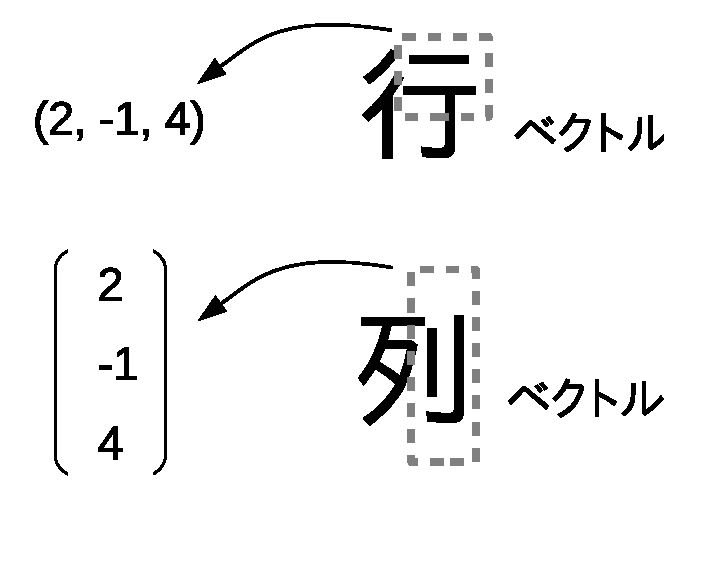
\includegraphics[width=7cm]{row_col.eps}
    \caption{数ベクトルの成分の並べ方\label{fig:row_col}}
\end{figure}
\hv

本章では, 特に理由の無い限り, 行ベクトルで書く。

さて, 座標(数ベクトル)を使うと, ベクトルの計算が楽にできる。まず, ベクトルのスカラー倍は, 
座標の各成分(座標を構成する個々の数値)をスカラー倍すればOK。
例えば${\bf a}=(2,\, -1,\, 3)$とすれば, ${\bf a}$の5倍は, 
\begin{eqnarray}
5{\bf a}&=&5(2,\, -1,\, 3)=(5\times2,\, 5\times(-1),\, 5\times3)\nonumber\\
        &=&(10,\, -5,\, 15)
\end{eqnarray}
である。

ベクトルどうしの和(足し算)は, 成分どうしの和でOK。例えば, 
${\bf a}=(2, -1, 4)$と${\bf b}=(1, 6, 0.2)$の和は, 
\begin{eqnarray*}
{\bf a}+{\bf b}&=&(2,\, -1,\, 4)+(1,\, 6,\, 0.2)\\
               &=&(2+1,\, -1+6,\, 4+0.2)
               =(3,\, 5,\, 4.2)
\end{eqnarray*}
である。\hv

\begin{q}\label{q:vect_2D_calc0} 2つのベクトル: ${\bf a}=(1,2)$, ${\bf b}=(2,3)$について, 
以下の数ベクトルを求めよ。
\begin{edaenumerate}
\item $2{\bf a}$
\item ${\bf a}-{\bf b}$
\end{edaenumerate}\end{q}
\hv

\begin{q}\label{q:vect_3D0_calc} 
${\bf a}=(1, 2, -1)$, ${\bf b}=(2, -1, -2)$について, 
$2{\bf a}$と$3{\bf a}-2{\bf b}$をそれぞれ求めよ。
\end{q}\hv

さて, \pref{eq:def_parallel}で学んだように, 
2つのベクトル${\bf a}$, ${\bf b}$が, 0でないスカラー$\alpha$によって, 
\begin{eqnarray}\alpha{\bf a}={\bf b}\end{eqnarray}
と書けるとき, ${\bf a}$と${\bf b}$は互いに\textgt{平行}である, 
という。例えば, $(1, 2)$と$(2, 4)$は, $2(1, 2)=(2, 4)$
と書けるから, 互いに平行である。\hv

\begin{q}\label{q:vect_3D0_parallel} 2つのベクトル: 
${\bf a}=(1, 2, 6)$, ${\bf b}=(x, y, -2)$について, 
が互いに平行なとき, $x$と$y$の値を求めよ。
\end{q}\vv


\section{ベクトルの大きさ}

ベクトル${\bf a}$の大きさを, $|{\bf a}|$と表す(縦棒で挟む)。

平面ベクトル$(x, y)$の大きさは, 
\begin{eqnarray}
|(x, y)|=\sqrt{x^2+y^2}\label{eq:vector_norm00}
\end{eqnarray}
である。これは三平方の定理から明らかだ。同様に, 
空間ベクトル$(x, y, z)$の大きさは, 
\begin{eqnarray}
|(x, y, z)|=\sqrt{x^2+y^2+z^2}\label{eq:vector_norm_3D}
\end{eqnarray}
である。\hv

\begin{q}\label{q:vector_norm2} 以下のベクトルの大きさを求めよ:
\begin{edaenumerate}<3>
\item $(1, 1, 1)$
\item $(3, -4)$
\item $(0, 0)$
\end{edaenumerate}\end{q}
\hv

\begin{q}\label{q:vect_length_scalar} 任意のベクトル${\bf a}$と
スカラー$\alpha$について, 次式を示せ:
\begin{eqnarray}
|\alpha{\bf a}|=|\alpha||{\bf a}|\label{eq:vect_scalar_absvalue}
\end{eqnarray}
\end{q}
\hv

大きさが0のベクトルを零ベクトルと言って, ${\bf 0}$と書く約束だった。
もし平面ベクトル$(x, y)$が零ベクトルなら, $|(x, y)|=\sqrt{x^2+y^2}=0$, 
すなわち, $x^2+y^2=0$である。これを満たすのは, $x=y=0$しかない。
つまり, 平面の零ベクトルは$(0, 0)$である。

同様に, 空間の零ベクトルは$(0,0,0)$である。\hv

大きさが1のベクトルを\underline{単位ベクトル} \index{たんいべくとる@単位ベクトル}
%(unit vector)
と呼ぶ。
\hv

\begin{q}\label{q:vect_unit} 
以下は全て単位ベクトルであることを示せ。ヒント: \eref{eq:vector_norm00}を使う。
(5)では\eref{eq:vect_scalar_absvalue}を使う。
\begin{enumerate}
\item $(1, 0)$
\item $(-1/\sqrt{2}, -1/\sqrt{2})$
\item $(1/\sqrt{3}, 1/\sqrt{3}, 1/\sqrt{3})$
\item 任意の実数$\theta$について, $(\cos\theta, \sin\theta)$
\item 零ベクトルでない任意のベクトル${\bf a}$について, ${\bf a}/|{\bf a}|$
\end{enumerate}
\end{q}
\vv


\section{内積}

2つのベクトル${\bf a}$, ${\bf b}$について, 成す角を$\theta$とするとき, 
\begin{eqnarray}
|{\bf a}||{\bf b}|\cos \theta\label{eq:def_inprod_00}
\end{eqnarray}
という量を, ${\bf a}$と${\bf b}$の\underline{内積} \index{ないせき@内積}
と呼び, ${\bf a}\bullet{\bf b}$と表す(定義)\footnote{内積は
「\underline{スカラー積}」\index{すからーせき@スカラー積}とも呼ばれる。}。\hv

この式から明らかなように, 内積の結果はスカラーである。
(ちなみに後で「外積」という演算が出てくるが, 外積の結果はベクトルである。)\hv

\begin{q}\label{q:vect_inprod_length2} 任意のベクトル${\bf a}$について次式を示せ:
\begin{eqnarray}
{\bf a}\bullet{\bf a}=|{\bf a}|^2
\end{eqnarray}
\end{q}\hv

\begin{q}\label{q:vect_inprod_perpendic} ${\bf 0}$でないベクトル${\bf a}$, ${\bf b}$について, 
\begin{eqnarray}
{\bf a}\bullet{\bf b}=0\label{eq_vect_inprod_rightangle}
\end{eqnarray}
ならば${\bf a}$と${\bf b}$は直交することを示せ。
\end{q}\hv

\begin{q}\label{q:vect_inprod_angle} ${\bf 0}$でないベクトル${\bf a}$, ${\bf b}$について, 
その成す角を$\theta$とするとき, 次式を示せ。
\begin{eqnarray}
\cos \theta=\frac{{\bf a}\bullet{\bf b}}{|{\bf a}||{\bf b}|}\label{eq:cos_inpro}
\end{eqnarray}\end{q}\hv

さて, 内積の定義(\eref{eq:def_inprod_00})には, 座標のことが書かれていない。
そこで, 座標で内積を計算するにはどうすればいいかを考えよう。まずとりあえず平面ベクトル
に関して考えよう。

${\bf a}=(a_1, a_2)$, ${\bf b}=(b_1, b_2)$とする。${\bf a}\bullet{\bf b}$が
どのように$a_1, a_2, b_1, b_2$で表されるかを知りたいのだ。そこで, 
${\bf a}$, ${\bf b}$をそれぞれ位置ベクトルとする点をA, Bとする。
三角形OABについて, 余弦定理より, 
\begin{eqnarray}
\text{AB}^2=\text{OA}^2+\text{OB}^2-2\text{OA}\,\,\text{OB}\,\cos\theta
\end{eqnarray}
が成り立つ(ここで$\theta$は角AOB, すなわち${\bf a}$と${\bf b}$がなす角)。これを変形して, 
\begin{eqnarray}
\text{OA}\,\,\text{OB}\,\cos\theta=\frac{\text{OA}^2+\text{OB}^2-\text{AB}^2}{2}\label{eq:inprod_coord06}
\end{eqnarray}
となる。OA$=|{\bf a}|$, OB$=|{\bf b}|$より, 上の式の左辺は${\bf a}\bullet{\bf b}$である。
右辺を座標で求めるために, まず, 
\begin{eqnarray}
&&\text{OA}^2=|{\bf a}|^2=a_1^2+a_2^2\\
&&\text{OB}^2=|{\bf b}|^2=b_1^2+b_2^2\\
&&\text{AB}^2=|\overrightarrow{\text{AB}}|^2=|{\bf b}-{\bf a}|^2\nonumber\\
&&=|(b_1-a_1, b_2-a_2)|^2=(b_1-a_1)^2+(b_2-a_2)^2\nonumber\\
&&=a_1^2+a_2^2+b_1^2+b_2^2-2(a_1b_1+a_2b_2)
\end{eqnarray}
である。これらを\eref{eq:inprod_coord06}の右辺に代入すると, 
\begin{eqnarray}
=\frac{2(a_1b_1+a_2b_2)}{2}=a_1b_1+a_2b_2
\end{eqnarray}
となる。従って, 
\begin{eqnarray}
{\bf a}\bullet{\bf b}=a_1b_1+a_2b_2\label{eq:def_inprod_05}
\end{eqnarray}
となる。なんと! 座標で内積を求めるには, 成分同士をかけて足すだけでいいのだ!
これは空間ベクトル(座標成分が3つある場合)でも同様である。すなわち, 
${\bf a}=(a_1, a_2, a_3)$, ${\bf b}=(b_1, b_2, b_3)$について, 
\begin{eqnarray}
{\bf a}\bullet{\bf b}=a_1b_1+a_2b_2+a_3b_3\label{eq:def_inprod_3D}
\end{eqnarray}
となる。\hv

\begin{q}\label{q:vect_inprod_coord_3D} \eref{eq:def_inprod_3D}を
導け。ヒント: \eref{eq:def_inprod_05}を導いたのとほぼ同じ手順。
\end{q}\hv


ここでは証明しないが, 内積には以下のような性質がある(${\bf a}, {\bf b}, {\bf a}_1, {\bf a}_2$は任意の
ベクトルであり, $\alpha$は任意のスカラー):
\begin{itembox}{内積の性質}
\begin{enumerate}
\item ${\bf a}\bullet{\bf a} \geq 0$
\item ${\bf a}\bullet{\bf a} = 0$となるのは${\bf a} = {\bf 0}$のときに限る。
\item ${\bf a}\bullet{\bf b} = {\bf b}\bullet{\bf a}$ 
\item $(\alpha{\bf a})\bullet{\bf b} = \alpha({\bf a}\bullet{\bf b})$
\item $({\bf a}_1+{\bf a}_2)\bullet{\bf b} = {\bf a}_1\bullet{\bf b}+{\bf a}_2\bullet{\bf b}$
\end{enumerate}
\end{itembox}
(1), (2), (3), (4)は定義から自明だろう。(5)は, \eref{eq:def_inprod_05}
を利用して成分で考えれば簡単に証明できる。\hv


\begin{q}\label{q:vect_inprod_coord2D} ${\bf a}=(1,2), {\bf b}=(2,3)$
について, ${\bf a}\bullet{\bf b}$を求めよ。
\end{q}
\hv

\begin{q}\label{q:vect_3D_inprod} ${\bf a}=(1, 2, -1)$, ${\bf b}=(3, -4, 5)$について, 
${\bf a}\bullet{\bf b}$を求めよ。
\end{q}\hv

\begin{q}\label{q:vect_inprod_angle_coord2D} ${\bf a}=(1,1), {\bf b}=(-1,3)$について, 成す角$\theta$の余弦, つまり$\cos \theta$を求めよ。
\end{q}\hv

\begin{q}\label{q:vect_inprod_shadow2D} 三角形OABを考える。Oを始点, Aを終点とするベクトルを${\bf a}$とし, 
Oを始点, Bを終点とするベクトルを${\bf b}$とする。いま, ${\bf b}$と同じ
方向で, 長さ1であるベクトル(単位ベクトル)を${\bf e}_b$とすると, 
\begin{eqnarray}
{\bf a}\bullet{\bf e}_b
\end{eqnarray}
は, Aから辺OBにおろした垂線の足Pと点Oの距離(ただし角AOBが鈍角の場合は負)
であることを示せ。これを, 「${\bf a}$から${\bf b}$に落とした
\underline{正射影\index{せいしゃえい@正射影}の長さ}」と呼ぶ。
\end{q}\hv

\begin{q}\label{q:vect_inprod_shadow2D1} ${\bf a}=(1,1), {\bf b}=(-1,3)$
について, ${\bf a}$から${\bf b}$に落とした正射影の長さを求めよ。
\end{q}\hv

\begin{q}\label{q:vect_inprod_trig_area} 三角形OABを考える。Oを始点, Aを終点とするベクトルを${\bf a}$とし, 
Oを始点, Bを終点とするベクトルを${\bf b}$とする。このような三角形を, 「${\bf a}$と${\bf b}$が張る三角形」という。
その面積を$s$とする。
\begin{enumerate}
\item 次式を示せ:
\begin{eqnarray}
s=\frac{1}{2}\sqrt{|{\bf a}|^2|{\bf b}|^2-({\bf a}\bullet{\bf b})^2}\label{eq:vect_inprod_trig_area1}
\end{eqnarray}
\item ${\bf a}=(a, b)$, ${\bf b}=(c, d)$とする。次式を示せ。
\begin{eqnarray}
s=\frac{|ad-bc|}{2}\label{eq:triangle_area2}
\end{eqnarray}
\item ${\bf a}=(1, 2)$, ${\bf b}=(3, 4)$のとき$s$を, 
\eref{eq:vect_inprod_trig_area1}と\eref{eq:triangle_area2}の
それぞれで求めよ。どちらが楽か?
\item ${\bf a}$と${\bf b}$の張る平行四辺形(${\bf a}$と${\bf b}$を2辺とする平行四辺形)の面積$S$について次式を示せ:
\begin{eqnarray}
S=|ad-bc|\label{eq:parallelogram}
\end{eqnarray}
\end{enumerate}\end{q}
\hv

問\ref{q:vect_inprod_trig_area}で見たように, 2つのベクトルが張る三角形の
面積を求める式は, \eref{eq:vect_inprod_trig_area1}と\eref{eq:triangle_area2}の
2つがある\footnote{これ以外にも様々な式がある。有名なのはヘロンの公式という
式であるが, ヘロンの公式はあまり実用的ではない。}。高校数学では
\eref{eq:vect_inprod_trig_area1}が有名だが, それを変形して
得られる\eref{eq:triangle_area2}や, その平行四辺形版である
\eref{eq:parallelogram}はほとんど出てこない。
しかし, 大学での数学では, \eref{eq:triangle_area2}や\eref{eq:parallelogram}は
後に学ぶ「行列式」という概念につながる, とても重要な式である。
それを抜きにしても, \eref{eq:triangle_area2}の方が
\eref{eq:vect_inprod_trig_area1}よりもずっと計算が楽だ。\hv

\begin{faq}{\small\textgt{なぜ高校では\eref{eq:triangle_area2}よりも
\eref{eq:vect_inprod_trig_area1}を使わせるのでしょうか?} ... 
ホントに謎ですね。一つありえるのは, \eref{eq:vect_inprod_trig_area1}は
空間ベクトル(成分が3つの場合)にも使えるけど, \eref{eq:triangle_area2}
は平面ベクトル(成分が2つ)にしか使えない, という理由です。
\eref{eq:triangle_area2}を空間に拡張することはできるのですが(それが
後で学ぶ「外積」というやつ), 高校では範囲外です。}\end{faq}\hv

\begin{freqmiss}{\small\textgt{内積をあらわす「$\bullet$」という記号を省略したり, 
$\times$という記号で代用してしまう} ... 
普通の数(スカラー)の積であれば, そのようなことは許されるけど, 
内積では許されません。内積は普通の数(スカラー)の積とは全く
別の概念。例えば, 普通の数$a, b$について, その積は, 
\begin{eqnarray*}
ab\quad\quad a\bullet b\quad\quad a\times b
\end{eqnarray*}
という3通りの書き方のいずれもが許され, これらは同じ意味です。
しかし, ベクトル${\bf a}, {\bf b}$について, 
\begin{eqnarray*}
{\bf a}{\bf b}\quad\quad{\bf a}\bullet{\bf b}\quad\quad{\bf a}\times{\bf b}
\end{eqnarray*}
という3つの式は, 意味が互いに違います。すなわち, ${\bf a}{\bf b}$という式は
意味がありません\footnote{ただし, 大学の数学ではテンソル積というものを
この式で表すこともある。}。${\bf a}\bullet{\bf b}$は内積を表します。${\bf a}\times{\bf b}$
は内積ではなく, 後に学ぶ「外積」というものを表します。}\end{freqmiss}\hv

\begin{faq}{\small\textgt{ベクトルは割り算はできないのですか?} ... 
ベクトル\textgt{を}スカラーで割ることはできます。しかし, スカラーやベクトルを
ベクトル\textgt{で}割ることはできません(定義されない, すなわち意味がない)。例えば
$(1, 2), (3, 4)$という2つのベクトルについて, $(1, 2)/(3, 4)$というような
「割り算」は不可能です。

\textgt{たとえば, $(2, 4)/(1, 2)=2$とかはダメですか?} ... 
言いたいことはわかる! でも, そういうのもやらないのです。その式は
$(2, 4)=2(1, 2)$と書けるし, それで十分です。}\end{faq}
\vv

\section{平面の中の直線と法線ベクトル}

すでに君は, 方程式
\begin{eqnarray}
ax+by+c=0\quad\text{($a, b, c$は実数の定数)}\label{eq:axbyc_line}
\end{eqnarray}
は, $xy$平面上で直線を表すことを知っているだろう(わからなければ, 
これを$y=$の式に変形してみればよい)。さて, ここで
面白い, そしてとても便利な事実がある。$x$と$y$の係数を並べて
できるベクトル$(a, b)$は, この直線に直交するのだ!

なぜかを考えよう。まず直線上の任意の2点: A$(x_0, y_0)$, B$(x_1, y_1)$
を考える。これらは次式を満たす:
\begin{eqnarray}
ax_0+by_0+c=0\\
ax_1+by_1+c=0
\end{eqnarray}
辺々引き算して, 
\begin{eqnarray}
a(x_1-x_0)+b(y_1-y_0)=0
\end{eqnarray}
となる。これは次式と同じことだ:
\begin{eqnarray}
(a, b) \bullet (x_1-x_0, y_1-y_0)=0
\end{eqnarray}
ここで, $(x_1-x_0, y_1-y_0)$は$\overrightarrow{\text{AB}}$である。
従って, $(a, b) \bullet \overrightarrow{\text{AB}}=0$となり, 
$(a, b)$は$\overrightarrow{\text{AB}}$と直交していることがわかる。
$\overrightarrow{\text{AB}}$は直線に沿った(直線に平行の)ベクトルなので, 
結局, この直線はベクトル$(a, b)$と垂直である。\qed\hv

一般に, 線や面に垂直なベクトルのことを
\underline{法線ベクトル}\index{ほうせんべくとる@法線ベクトル} (normal vector)という。
$(a, b)$は, 直線$ax+by+c=0$の法線ベクトル(のひとつ)である。\hv

\begin{q}\label{q:vect_line2D0} $(1, 2)$を通り, ベクトル$(3, -1)$
に垂直な直線を表す式を示せ。(ヒント: 法線ベクトル(の一つ)が
$(3, -1)$とわかっているので, 求める式は$3x-y+c=0$のような形に書ける。
あとは$c$を決めればOK)\end{q}\hv

\begin{exmpl}\label{exmpl:line_normal_2D} 
点$(2, 1)$を通り, ベクトル$(3, -5)$に平行な直線を表す式は? 
まず法線ベクトルを求めよう。それには$(3, -5)$に垂直なベクトル(内積したら0
になるベクトル)をテキトーに決めればよい。$(5, 3)$がそうだ。これが直線の
法線ベクトルだから, 求める直線の式は$5x+3y+c=0$の形に書けるだろう($c$は未知の定数)。これに
点$(2, 1)$を入れると, $13+c=0$, よって$c=-13$。よって, 求める式は, 
$5x+3y-13=0$\qed
\end{exmpl}\hv

\begin{q}\label{q:vect_line2D1} $(1, 2)$を通り, 
ベクトル$(1, -1)$に平行な直線を表す式を示せ。
(ヒント: 上の例を参考に!)
\end{q}\hv


\begin{faq}{\small\textgt{例\ref{exmpl:line_normal_2D}
で, 法線ベクトルを「テキトーに」決めましたが, そんなんでいいのですか? 
法線ベクトルは他にもありえますよね。} ... その通り。法線ベクトルは
$(5, 3)$以外にもたくさんあります。でも, どの法線ベクトルも互いに
平行なので, $(5, 3)$の何倍か, つまり$k(5, 3)$という形
で表されます($k$は0以外の任意の実数)。それを使って, 直線の式を
$5kx+3ky+c'=0$と表し($c'$は$c$とは別の未知数), 
$(2, 1)$をこれに代入すれば, $c'=-13k$になり, 直線の式は
$5kx+3ky-13k=0$となります。両辺を$k$で割れば, 結局同じ式が
出てきます。というわけで, 法線ベクトルは, (零ベクトルでさえなければ)
本当にテキトーに決めていいのです。どんなふうに決めても, 結論は
一緒です。}\end{faq}\vv



\section{空間の中の平面と法線ベクトル}

前節で考えた平面の中の直線の話は, 空間の中の平面の話に拡張できる。まず, 次式を考えよう:

\begin{eqnarray}
ax+by+cz+d=0\,\,\,\,\,\, (a, b, c, d\text{は実数の定数})\nonumber\\\label{eq:plane_ax_by_cz_d}
\end{eqnarray}

これは\eref{eq:axbyc_line}, すなわち平面内の直線の式に似ている。実は\eref{eq:plane_ax_by_cz_d}
は, 空間内の平面を表す式であり, $(a, b, c)$はその平面の法線ベクトルなのだ!

そのことを今から示そう。まず, \eref{eq:plane_ax_by_cz_d}を満たす
任意の2点: A$(x_0, y_0, z_0)$, B$(x_1, y_1, z_1)$を考える。当然ながら次式が成り立つ:
\begin{eqnarray}
ax_0+by_0+cz_0+d=0 \\
ax_1+by_1+cz_1+d=0\label{eq:vect_plane_inprod2}
\end{eqnarray}
両辺引き算して, 
\begin{eqnarray}
a(x_1-x_0)+b(y_1-y_0)+c(z_1-z_0)=0
\end{eqnarray}
これは次式と同じことである:
\begin{eqnarray}
(a, b, c) \bullet (x_1-x_0,\, y_1-y_0,\, z_1-z_0)=0\label{eq:vect_plane_inprod4}
\end{eqnarray}
ここで, 明らかに$(x_1-x_0,\, y_1-y_0,\, z_1-z_0)=\overrightarrow{\text{AB}}$である。
また, ベクトル$(a, b, c)$を${\bf n}$と置く。すると\eref{eq:vect_plane_inprod4}は, 
\begin{eqnarray}
{\bf n} \bullet \overrightarrow{\text{AB}}=0\label{eq:vect_plane_inprod6}
\end{eqnarray}
となる。つまり, ${\bf n}$と$\overrightarrow{\text{AB}}$は互いに
直交する。これの意味するところは何だろうか?
今, 点Aを固定して考える。Bはいろんな点を動くことが
できるのだが, \eref{eq:vect_plane_inprod6}に
よると, 固定点Aから点Bへのベクトルが, ひとつのベクトル${\bf n}$と
必ず直交していなければならない。そのような点Bの「動ける範囲」は, 
点Aを通る平面で, なおかつ${\bf n}$に垂直な平面である (直感的にわかるだろう)。
つまり, \eref{eq:plane_ax_by_cz_d}は, 3次元空間の中の平面を表す方程式であり, 
$x$と$y$と$z$の係数を並べてできるベクトル${\bf n}=(a, b, c)$は, この平面の法線ベクトルである。\hv

\begin{q}\label{q:vect_3D1}
$(0, 0, 1)$を通り, ベクトル$(1, 2, -1)$に垂直な平面の方程式を求めよ。
\end{q}
\hv

ここまでは, 前節でやった, 平面内の直線の話と大きくは違わない。
上の問も, 問\ref{q:vect_line2D0}と似たようなものだ。しかし, 
例\ref{exmpl:line_normal_2D}や問\ref{q:vect_line2D1}の
ように, 「なんちゃらに平行な直線を求めよ」の平面版はどうだろう?
例えば, 「$(0,0,0)$を通り, ベクトル$(1,0,0)$に平行な平面を
求めよ」みたいな問題はどうだろう?

これは困る。解けないのだ。なぜかというと, 「$(0,0,0)$を通り, 
ベクトル$(1,0,0)$に平行な平面」というのはたくさんあって, 
一つに決まらないのだ。これは要するに「原点を通り, $x$軸に平行
な平面」ということだから, 例えば「$x$軸と$y$軸を含む平面」や, 
「$x$軸と$z$軸を含む平面」や, その中間など, たくさんある。
「ひとつのベクトルに平行」という条件だけでは, 平面の向きは
決まらないのだ。

しかし, 「ふたつのベクトルのどちらにも平行」という条件なら平面
の向きは決まる。例えば, 「$(0,0,0)$を通り, 2つのベクトル$(1,0,0)$
と$(0,1,0)$に平行な平面」と言われれば, 「$x$軸と$y$軸を含む平面」
に決まる(式で書けば$z=0$)。

では, 次の問題をやってみよう:

\begin{q}\label{q:vect_3D_2vecpara_plane}
$(0,0,1)$を通り, 2つのベクトル${\bf a}=(1, 1, -3)$, 
${\bf b}=(1, 2, 1)$の両方に平行な平面を求めよう。
まず法線ベクトルを${\bf n}=(p, q, r)$と置く。($p, q, r$は未知の定数)
\begin{enumerate}
\item 次式を示せ: $p+q-3r=0$ (ヒント: ${\bf n}$と${\bf a}$が垂直)
\item 次式を示せ: $p+2q+r=0$ (ヒント: ${\bf n}$と${\bf b}$が垂直)
\item $p$と$q$を$r$だけで表わせ。
\item $(p, q, r)=r(7, -4, 1)$であることを示せ。(これで法線ベクトルが求まった!)
\item 平面を表す式を求めよ。
\end{enumerate}
\end{q}

難しくはないが, そこそこ面倒である。次の節で, もっと簡単にできる, 
魔法のような道具を紹介する。
\vv


\section{外積}
2つの3次元の数ベクトル
\begin{equation}
{\bf a}=
\begin{bmatrix}
a_1\\
a_2\\
a_3\\
\end{bmatrix},\,\,\,\,
{\bf b}=
\begin{bmatrix}b_1\\
b_2\\
b_3\\
\end{bmatrix}\label{eq:vectprod0}\end{equation}
から, 以下のように別の3次元の数ベクトルを導き出す
操作を${\bf a}$と${\bf b}$の\underline{外積} \index{がいせき@外積}または「ベクトル積」
\index{べくとるせき@ベクトル積}と呼び, ${\bf a}\times{\bf b}$と書く。
すなわち, 
\begin{eqnarray}
{\bf a}\times{\bf b}=
\begin{bmatrix}a_1\\
a_2\\
a_3\\
\end{bmatrix}\times
\begin{bmatrix}b_1\\
b_2\\
b_3\\
\end{bmatrix}:=
\begin{bmatrix}a_2b_3-a_3b_2\\
a_3b_1-a_1b_3\\
a_1b_2-a_2b_1\\
\end{bmatrix}\label{eq:vectprod}
\end{eqnarray}
と定義する。例えば, ${\bf a}=(1, 2, 3)$, ${\bf b}=(4, 5, 6)$の場合, 
\begin{eqnarray}
{\bf a}\times{\bf b}=
\begin{bmatrix}1\\
2\\
3\\
\end{bmatrix}\times
\begin{bmatrix}4\\
5\\
6\\
\end{bmatrix}=
\begin{bmatrix}2\times6-3\times5\\
3\times4-1\times6\\
1\times5-2\times4\\
\end{bmatrix}
=\begin{bmatrix}-3\\
6\\
-3\\
\end{bmatrix}\nonumber\\\label{eq:vectprod_ex1}
\end{eqnarray}
となる。\hv

\begin{faq}{\small\textgt{こんなのややこしくて覚えられません!}
... 誰もが最初はそう思います。でも慣れれば大丈夫。まず\eref{eq:vectprod_ex1}
を何回か紙の上で再現して, 外積の計算に慣れてください。}\end{faq}\hv

\begin{freqmiss}{\small\textgt{\eref{eq:vectprod}の右辺を, 
\begin{eqnarray}
\begin{bmatrix}
a_1b_2-a_2b_1\\
a_2b_3-a_3b_2\\
a_3b_1-a_1b_3\\
\end{bmatrix}
\text{とか, }
\begin{bmatrix}
a_3b_1-a_1b_3\\
a_2b_3-a_3b_2\\
a_1b_2-a_2b_1\\
\end{bmatrix}
\end{eqnarray}
と間違える。} .... 成分の順番に注意してください。
外積の結果の$x$成分($a_2b_3-a_3b_2$)は, もとの
ベクトルの$y$成分($a_2$や$b_2$)と$z$成分($a_3$や$b_3$)
から求まります。同様に, $y$成分はもとのベクトルの$z$成分と$x$成分から, 
$z$成分はもとのベクトルの$x$成分と$y$成分から
もとまるのです。また, 同じ位置の成分どうしの
掛け算($a_2\,b_2$とか)は現れません。
「求めたい成分以外の成分で計算する。自分とは違う位置の成分と掛ける」
と覚えておきましょう。}\end{freqmiss}\hv

\begin{freqmiss}{\small\textgt{外積と内積を混同してしまう。外積を求めよ, 
という問に内積を答えたり, その逆をしたり} ... 外積と内積は
全く別物! それぞれの定義を確認しよう。}\end{freqmiss}\hv

\begin{freqmiss}{\small\textgt{外積を表す"$\times$"という記号を, 省略したり
"$\bullet$"という記号で代用してしまう} ... それはダメ。
"$\times$"と"$\bullet$"の混用や省略が許されるのは, 
数どうしの積だけ。それ以外の「積」, すなわちベクトルの内積や外積, 
行列の積, 集合の直積などは, 数どうしの積とは根本的に違うもの
なので, それぞれに決まった書き方を守らねばなりません。}\end{freqmiss}\hv


さて, この外積はなかなか強いヤツである。

\begin{q}\label{q:vectprod_inprod} 
\begin{enumerate}
\item \eref{eq:vectprod}において, 次式を証明せよ:
\begin{eqnarray}
({\bf a}\times{\bf b})\bullet{\bf a}=0\\
({\bf a}\times{\bf b})\bullet{\bf b}=0
\end{eqnarray}
\item それが実際に\eref{eq:vectprod_ex1}において
成り立っていることを確認せよ。
\end{enumerate}
\end{q}

すなわち, 次の定理が成り立つ:\hv

外積の定理1) ${\bf a}\times{\bf b}$は, ${\bf a}$と${\bf b}$の両方に垂直である。\hv

てことは, 問\ref{q:vect_3D_2vecpara_plane}ではわざわざ方程式を
解いて求めた法線ベクトルが, 一発で求まるのだろうか? それをやってみよう:

\begin{q}\label{q:vect_3D_2vecpara_plane2} 問\ref{q:vect_3D_2vecpara_plane}
の${\bf a}=(1, 1, -3)$, ${\bf b}=(1, 2, 1)$について, ${\bf a}\times{\bf b}$
を計算せよ。\end{q}\hv

注: 「外積の定理1」は外積の計算結果のチェックに便利である。例えば, 
\eref{eq:vectprod_ex1}について, 
もとの2つのベクトルと内積をとって0になることを確かめるのだ:
\begin{eqnarray*}
&&\begin{bmatrix}1\\
2\\
3\\
\end{bmatrix}\bullet
\begin{bmatrix}-3\\
6\\
-3\\
\end{bmatrix}=-3+12-9=0\\
&&\begin{bmatrix}4\\
5\\
6\\
\end{bmatrix}\bullet
\begin{bmatrix}-3\\
6\\
-3\\
\end{bmatrix}=-12+30-18=0
\end{eqnarray*}

首尾よく0になっていて, 一安心である。0になったからといって計算が正しいとまでは言えない, 
0にならなければ, どこかで必ず計算ミスをしている。\hv

というわけで, 外積は便利だ。しかもこれは外積の強さのまだ一部だ。
もっとすごいのは次の定理だ:\hv

外積の定理2) $|{\bf a}\times{\bf b}|$は${\bf a}$と${\bf b}$
が張る平行四辺形の面積に等しい\footnote{それは$|{\bf a}||{\bf b}|\sin\theta$でもある
($\theta$は${\bf a}$と${\bf b}$のなす角)。}。\hv

これは, \eref{eq:parallelogram}を拡張したものと言える。
証明はちょっとめんどくさいので, 章末の演習問題にまわす。
この定理を使う問題を解いてみよう:\hv

\begin{q}\label{q:univ_vectprod0} 以下の各場合について, 
${\bf a}\times{\bf b}$を求め, ${\bf a}, {\bf b}$
の張る平行四辺形の面積を求めよ。
\begin{enumerate}
\item ${\bf a}=(1, 2, 0),\,\,\, {\bf b}=(1, 1, -1)$
\item ${\bf a}=(1, 0, 1),\,\,\, {\bf b}=(-1, 1, 2)$
\end{enumerate}\end{q}\hv

他にも, こういう定理がある:\hv

外積の定理3) 外積の順序を変えると符号が反転する。すなわち, 
\begin{eqnarray}
{\bf b}\times{\bf a}=-{\bf a}\times{\bf b}\label{eq:vectprod_order}
\end{eqnarray}

\begin{q}\label{q:vectprod_order} \eref{eq:vectprod_order}を
証明せよ。ヒント: \eref{eq:vectprod}の${\bf a}$と${\bf b}$を
ひっくり返して計算してみよう。\end{q}\hv

\begin{q}\label{q:vectprod_same} 任意のベクトル${\bf a}$について, 
次式が成り立つことを示せ:
\begin{eqnarray}
{\bf a}\times{\bf a}={\bf 0}\label{eq:vectprod_same}
\end{eqnarray}
ヒント: \eref{eq:vectprod_order}の${\bf b}$を${\bf a}$にすると...?\end{q}
\hv

さて, ここでは証明はしないが, もうひとつ, 以下のような定理がある
(図\ref{fig:vector_prod}も参照!):\\

外積の定理4) ${\bf a}\times{\bf b}$は, ${\bf a}$から${\bf b}$に右ネジをまわすときにネジが進む方を向く
\footnote{ただしこれは, $x$軸から$y$軸に向けて右ネジをまわすときにネジが進む方を$z$軸が向いている場合。}。\\
\begin{figure}
    \centering
      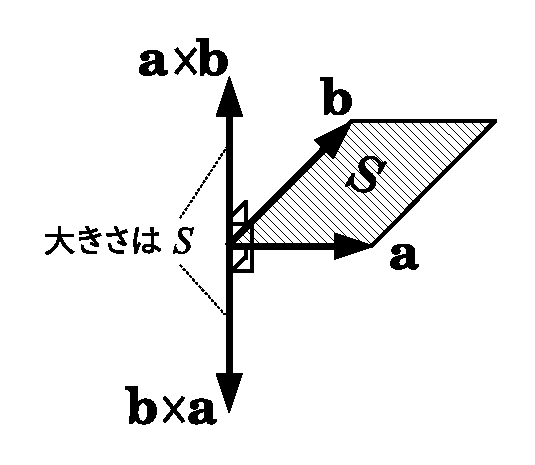
\includegraphics[width=7cm]{vector_prod.eps}
      \caption{外積(ベクトル積)の幾何学的な概念図。${\bf a}\times{\bf b}$と${\bf b}\times{\bf a}$は, ともに
${\bf a}, {\bf b}$が張る平行四辺形の面積$S$をその大きさとするベクトルで, ${\bf a}, {\bf b}$の両方に
垂直。ただし, ${\bf a}\times{\bf b}$と${\bf b}\times{\bf a}$は互いに逆方向。
${\bf a}$から${\bf b}$に右ネジをまわすときにネジが進む側にあるのが${\bf a}\times{\bf b}$。
\label{fig:vector_prod}}    
\end{figure}\hv

\begin{faq}{\small\textgt{右ネジって何ですか?}
... ネジとかボルトはわかりますね。あれをドライバーで回すと, 
穴に入って行ったり穴から出てきたりするでしょ? 世の中のほとんど
のネジは, ドライバーを右に(つまり時計回りに)まわすと, ネジは
穴に入っていきます。それが右ネジです。ごく稀に, 逆, つまり左に
まわすと入っていくネジもあり, そういうのは左ネジ。}\end{faq}\hv

\begin{q}\label{q:univ_vectprod2} ${\bf e}_1=(1, 0, 0),\,\, {\bf e}_2=(0, 1, 0),\,\, {\bf e}_3=(0, 0, 1)$とすると, 
以下の式が成り立つことを示せ:
\begin{eqnarray}
&&{\bf e}_1\times{\bf e}_2={\bf e}_3\\
&&{\bf e}_2\times{\bf e}_3={\bf e}_1\\
&&{\bf e}_3\times{\bf e}_1={\bf e}_2\\
&&({\bf e}_1\times{\bf e}_1)\times{\bf e}_2={\bf 0}\\
&&{\bf e}_1\times({\bf e}_1\times{\bf e}_2)=-{\bf e}_2
\end{eqnarray}
\end{q}
\vspace{0.3cm}

\begin{q}\label{q:univ_vectprod3} 任意の空間ベクトル${\bf a}, {\bf b}, {\bf c}$と
任意の実数$p$に関して, 以下の式が成り立つことを, 外積の定義に戻って示せ:
\begin{eqnarray}
&&(p{\bf a})\times{\bf b}=p({\bf a}\times{\bf b})\label{eq:vectprod_scalar}\\
&&({\bf a}+{\bf b})\times{\bf c}={\bf a}\times{\bf c}+{\bf b}\times{\bf c}\label{eq:vectprod_bumpai}
\end{eqnarray}
\end{q}\hv

\begin{q}\label{q:scalar3prod_style} スカラー$p$と, 空間ベクトル${\bf a}, {\bf b}, {\bf c}$について, 
${\bf a}\bullet{\bf b}\times{\bf c}$や${\bf a}\times{\bf b}\times{\bf c}$という式は, 書き方がダメである。しかし, $p{\bf b}\times{\bf c}$という式は, 書き方の問題はない。これらはなぜか?
\end{q}\hv


\begin{faq}{\small\textgt{外積と内積の違いがわかりません。}\\
... 定義が全く違います。その他に端的な違いとして, 
\begin{itemize}
\item 内積の結果はスカラーだが, 外積の結果はベクトル。
\item 内積は順序を入れ替えても結果は変わらないが, 外積は順序を入れ替えると符号が反転する。
\item 内積は平面ベクトルでも空間ベクトルでも存在するが, 外積は空間ベクトルだけに存在する。
\item 内積は$ab\cos\theta$だが, 外積\textgt{の大きさ}は$ab \sin\theta$。
\end{itemize}
などが挙げられます(全て定義から導出可能)。}\end{faq}
\hv


\section{物理学とベクトル}

さて, 微積分と並んでベクトルは物理学で重要なツールだ。
速度や加速度や力などはベクトルを使って表現する。例として円運動を考えてみよう。

\begin{q}\label{q:vect_velocac2D1} $xy$座標平面上で, 原点を中心とする半径$r$の円周上を, 左回りに回転運動
する点Pを考える。時刻$t=0$のときPの位置は$(r,0)$であったとする。すると, 
時刻$t$のとき, 点Pの位置は, 以下の位置ベクトル${\bf r}(t)$であらわされる($r, \omega$は定数):
\begin{eqnarray}
{\bf r}(t)=(r\cos\omega t, r\sin\omega t)
\end{eqnarray}
これは, 原点からの距離$r$を保ったまま, $x$軸から左回りに角$\omega t$
だけ回転した位置である(\pref{sect:polar_coord_2D}の極座標!)。
このように, ある点(ここでは原点)からの距離が一定で, ある方向(ここでは$x$軸)からの
角が時間に比例して変化するような回転運動を, 「等速円運動」\index{とうそくえんうんどう@等速円運動}と言う。
このとき$\omega$を\underline{角速度} \index{かくそくど@角速度}と呼ぶ。
\begin{enumerate}
\item Pの速度${\bf v}(t)$と, その大きさを求めよ。
\item Pの加速度${\bf a}(t)$と, その大きさを求めよ。
\item 位置ベクトルと速度は直交していることを示せ(ヒント:内積)。
\item 速度ベクトルと加速度は直交していることを示せ。
\item 位置ベクトルと加速度は平行で逆向きであることを示せ。
\item 角速度が2倍になると, 速度や加速度の大きさはそれぞれ何倍になるか? 
\end{enumerate}\end{q}
\hv

こんなかんじで, ちょっとした運動を考えるだけでも, ベクトルとその微分が
ガンガン出てくる。\hv

\begin{faq}{\small\textgt{問\ref{q:vect_velocac2D1}(1)で, 
\begin{eqnarray*}v(t)=(-r\omega\sin\omega t, r\omega\cos\omega t)\end{eqnarray*}
と答えたら不正解でした。微分は間違っていないし, どこがダメなのですか?}
... ベクトルは太字。$v(t)$でなくて${\bf v}(t)$と書いて下さい。}\end{faq}
\hv

\begin{faq}{\small\textgt{$v(t)$を${\bf v}(t)$と書きなおしたけどまた不正解でした。}
... 答は合っていても, 導出過程が書かれていなければ正解にはできません。
${\bf v}(t)={\bf r}'(t)$と書いて(${\bf r}$は太字ですよ!), 
それに続けて上の式の右辺を書けばよいのです。}\end{faq}
\hv

\begin{faq}{\small\textgt{導出過程はどこまで詳しく書けばよいのでしょう?}
... 一概には言えませんが... 数学は定義から始まって, いくつも定理を重ねて
結論を導出します。だから, どの問題にも, そこに至るまでいくつかのステップがあるはず。その
ステップの最初の方はある程度省略してOKですが, 最後のほうのステップは省略してはいけません。
上の質問の例では, 速度を問われる問題なのだから, 速度をどう導出したか, という
ステップ(位置ベクトルを微分すること)は省略できない。でも, $r\cos\omega t$を
微分したらなぜ$-r\omega\sin\omega t$になるか, というところまでは遡る必要はありません。}\end{faq}\hv


内積も物理で使う。それは「仕事」だ。\pref{sect:energy_pressure}で
(というか中学校で)学んだように, 物体に力をかけて移動させるとき, 力と, 
その力の方向に動いた距離との積を, 「仕事」という。これは, 実はベクトルの内積で
表現すべきことなのだ。それを説明しよう。

移動前と移動後のそれぞれの位置ベクトルを${\bf r}_0$, ${\bf r}_1$とすると, 
$\Delta{\bf r}:={\bf r}_1-{\bf r}_0$は「移動した方向と距離」を持つ
ベクトルである。そういうのを「変位ベクトル」とか, 単に「変位」
という。また, かかる力を${\bf F}$とする。$\Delta{\bf r}$と${\bf F}$
のなす角を$\theta$と呼ぼう。すると, 「その力の方向に動いた距離」
は, $\Delta{\bf r}$を${\bf F}$に落とした正射影の長さであり, 
それは, $|\Delta{\bf r}|\cos\theta$である。従って, 
仕事は, $|{\bf F}|\,|\Delta{\bf r}|\cos\theta$となる...
ちょっと待て! それって, 結局, ${\bf F}\bullet\Delta{\bf r}$じゃないか!
そうなのだ。仕事とは, 要するに「力と変位の内積」なのだ。
「仕事=力かける距離」とよく言うが, その「かける」は内積なのだ。\\

外積も物理で使う。以下のような物理量は, 外積を使わないと表現できない:
\begin{itemize}
\item 力のモーメント(トルク): ${\bf r}\times{\bf F}$\index{ちからのもーめんと@力のモーメント}\index{とるく@トルク}
\item 角運動量: ${\bf r}\times{\bf p}$\index{かくうんどうりょう@角運動量}
\item 磁力: $q{\bf v}\times{\bf B}$\index{じりょく@磁力}
\end{itemize}

ここで, ${\bf r}$は質点の位置ベクトル, ${\bf F}$は質点にかかる力, ${\bf p}$は
質点の運動量(=質量と速度の積)\index{うんどうりょう@運動量}, $q$は電荷量, 
${\bf B}$は磁束密度\index{じそくみつど@磁束密度}という量である。\hv

これらの量や式が意味するところは, いずれ「物理学」で学ぶだろう。その準備のためにも, 
今ここで, 外積についてしっかり学んでおこう。

\begin{faq}{\small\textgt{中3のとき「右ネジの法則」を習いましたが, 外積と
関係あるのですか?} ... フレミングの法則ですね。そういうのは本来, 全て外積
で書くものです。それを理解すれば, 親指が何で人差し指が何で...と覚える必要
ありません。また, 「てこの原理」も外積で書けます。}\end{faq}
\hv

\begin{q}\label{q:vect_prod_diff} 2つのベクトル: 
\begin{eqnarray*}
{\bf a}(t)=
\begin{bmatrix}
a_1(t)\\
a_2(t)\\
a_3(t)\\
\end{bmatrix},\,\,\,
{\bf b}(t)=
\begin{bmatrix}
b_1(t)\\
b_2(t)\\
b_3(t)\\
\end{bmatrix}
\end{eqnarray*}
が, ともに変数$t$の関数であるとする。以下の式を証明せよ:
\begin{eqnarray}
&&({\bf a}\bullet{\bf b})'={\bf a}'\bullet{\bf b}+{\bf a}\bullet{\bf b}'\label{eq:inprod_diff}\\
&&({\bf a}\times{\bf b})'={\bf a}'\times{\bf b}+{\bf a}\times{\bf b}'\label{eq:vecprod_diff}
\end{eqnarray}
ヒント: $({\bf a}\bullet{\bf b})$や$({\bf a}\times{\bf b})$を成分で表して, 
愚直に積の微分の公式を適用していけばよい。
\end{q}
\hv



\section{ベクトルの応用}

科学では「重心」という言葉をよく耳にする。重心は, 感覚的には, 
物体を1点で支える時, その点で支えれば重力がバランスして, 傾いたり
転げ落ちたりしないような点のことである。実は, そういうのを含むような
きちんとした数学的な定義がある。それがこれだ:

物体を$n$個の質点(質量はあるが形や大きさの無い点)が構成する時, 
\begin{eqnarray}
{\bf G}:=\frac{m_1{\bf r}_1+m_2{\bf r}_2+\cdots+m_k{\bf r}_k+\cdots+m_n{\bf r}_n}{m_1+m_2+\cdots+m_k+\cdots+m_n}\nonumber\\
\end{eqnarray}
を位置ベクトルにとるような点を重心という(定義)。ここで, $m_k$は$k$番目の質点の質量, 
${\bf r}_k$は$k$番目の質点の位置ベクトルである。

このように定義された点で物体を支えると物体は転ばないことは, 数学的に証明できる。

\begin{exmpl} 同じ質量$m$の4個の質点(位置ベクトルをそれぞれ${\bf r}_1$〜${\bf r}_4$とする)
がつながってできている物体を考える。その重心の位置ベクトルは, 
\begin{eqnarray}
{\bf G}:=\frac{m{\bf r}_1+m{\bf r}_2+m{\bf r}_3+m{\bf r}_4}{m+m+m+m}\nonumber\\
=\frac{{\bf r}_1+{\bf r}_2+{\bf r}_3+{\bf r}_4}{4}\label{vect_gravcent4}
\end{eqnarray}
となる。\end{exmpl}

\begin{exmpl} 異なる質量を持つ2個の質点がつながってできている物体を考える。
質点1の質量と位置ベクトルを$m_1$, ${\bf r}_1$とし, 
質点2の質量と位置ベクトルを$m_2$, ${\bf r}_2$とする。重心の位置ベクトルは, 
\begin{eqnarray}
{\bf G}:=\frac{m_1{\bf r}_1+m_2{\bf r}_2}{m_1+m_2}
\end{eqnarray}
となる。これを\eref{eq:vect_naibun}と比べると, この重心は, 
質点1と質点2を結ぶ線分を, $m_2:m_1$の比に内分する点だとわかる。(例おわり)
\end{exmpl}
\hv

さて, 重心を利用して, 化学で出てくる重要な問題を解いてみよう。

正四面体は, 有機物を作る骨格, つまり炭素原子の配位に関する最も単純な幾何学的モデルであり, 
タンパク質や糖類などの巨大分子の機能や性質は, その立体的な幾何学構造から理解される。ベクトルを使って, 
正四面体の中心から頂点に伸びる線分どうしのなす角の大きさ(正四面体角\index{せいしめんたいかく@正四面体角})
を求めてみよう。

\begin{q}\label{q:vect_tetrahedron} 図\ref{fig:tetrahedron}のような正四面体を考える。
一つの頂点を原点Oとし, 残りの3つの頂点を点A, 点B, 点Cとする。
一辺の長さを$L$とする。すなわち, OA=OB=OC=AB=BC=CA=$L$である。この正四面体の各頂点に
同じ質量の質点があると考え, その重心を点Gとする。\eref{vect_gravcent4}から, 
\begin{eqnarray}
\overrightarrow{\text{OG}}=\frac{\overrightarrow{\text{OA}}+\overrightarrow{\text{OB}}+\overrightarrow{\text{OC}}}{4}\label{eq:vect_tetrahedron02}
\end{eqnarray}
である。
\begin{enumerate} 
\item 次式を示せ:
\begin{eqnarray}
\overrightarrow{\text{OA}}\bullet\overrightarrow{\text{OB}}=\overrightarrow{\text{OB}}\bullet\overrightarrow{\text{OC}}=\overrightarrow{\text{OC}}\bullet\overrightarrow{\text{OA}}=\frac{L^2}{2}\quad\quad\quad\quad
\label{eq:vect_tetrahedron04}
\end{eqnarray}
(ヒント: 三角形OABは一辺$L$の正三角形)
\item \eref{eq:vect_tetrahedron02}, \eref{eq:vect_tetrahedron04}を使って次式を示せ:
\begin{eqnarray}
\text{OG}=\frac{\sqrt{6}}{4}L\label{eq:vect_tetrahedron06}
\end{eqnarray}
(ヒント: まず\eref{eq:vect_tetrahedron02}を使って$\overrightarrow{\text{OG}}\bullet\overrightarrow{\text{OG}}$を計算する。
\item 正四面体角を$\theta$とする。\eref{eq:vect_tetrahedron06}を使って次式を示せ:
\begin{eqnarray}
\overrightarrow{\text{GO}}\bullet\overrightarrow{\text{GA}}=\frac{3}{8}L^2\cos\theta\label{eq:vect_tetrahedron08}
\end{eqnarray}
(ヒント: 内積の定義を素直に使う。GO=GAに注意せよ。)
\item 次式を示せ:
\begin{eqnarray}
\overrightarrow{\text{GA}}=\frac{3\overrightarrow{\text{OA}}-\overrightarrow{\text{OB}}-\overrightarrow{\text{OC}}}{4}\label{eq:vect_tetrahedron10}
\end{eqnarray}
(ヒント: $\overrightarrow{\text{GA}}=\overrightarrow{\text{OA}}-\overrightarrow{\text{OG}}$)
\item \eref{eq:vect_tetrahedron02}, \eref{eq:vect_tetrahedron10}を使って次式を示せ:
\begin{eqnarray}
\overrightarrow{\text{GO}}\bullet\overrightarrow{\text{GA}}=-\frac{L^2}{8}\label{eq:vect_tetrahedron12}
\end{eqnarray}
(ヒント: $\overrightarrow{\text{GO}}=-\overrightarrow{\text{OG}}$)
\item \eref{eq:vect_tetrahedron08}, \eref{eq:vect_tetrahedron12}を使って, $\cos\theta$の値を
求めよ。
\item 関数電卓を使って, $\theta$の値を, ラジアンと度分秒で表せ。
\end{enumerate}\end{q}
\begin{figure}
    \centering
    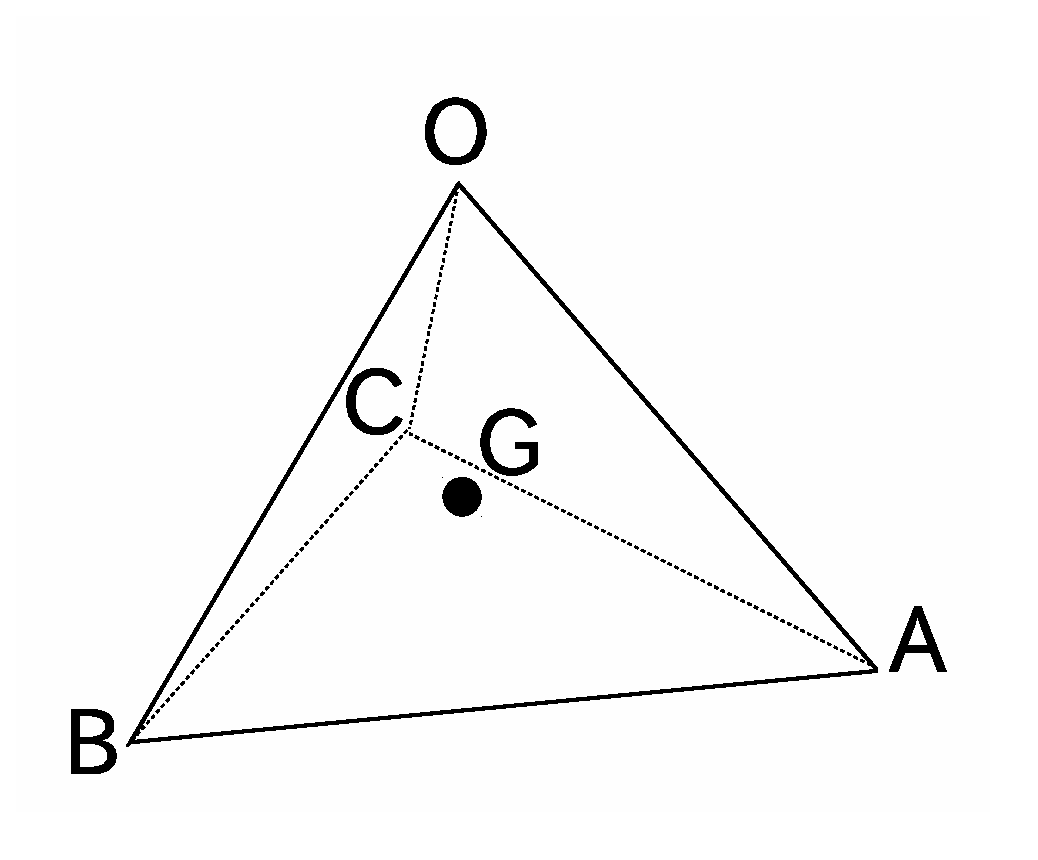
\includegraphics[width=7cm]{tetrahedron2.eps}
    \caption{正四面体OABC。問\ref{q:vect_tetrahedron}参照。\label{fig:tetrahedron}}
\end{figure}
\hv

ベクトルの応用例をもうひとつ(しかも全く違う話題)やってみよう。

\begin{q}\label{q:vect_wind2D} ある農地において, 防風林(風を遮るために農地近辺に作られる林)を造成するために, 
気象観測を行った。その結果, 風向と風速に関する, 以下の表のようなデータを得た。風は主にどちら
の方向から吹いていたか?
\begin{table}[!htb]\caption{ある日の風向風速観測結果}
\begin{center}
\begin{tabular}{ccc}\hline
時刻 & 風向(北からの角度) & 風速(m/s) \\  \hline
00:00 & 15& 3.0\\
06:00 & 40& 5.2\\
12:00 & 320& 1.5\\
18:00 & 260& 2.0\\  \hline
\end{tabular}
\end{center}
\end{table}
\small{ヒント: 風向と風速は, 一種の極座標である(\eref{eq:2Dpolar})。各時刻の風を
ベクトルとしてあらわし, その成分を平均する。電卓等を使うこと。
なお, 一般的に, 「風向」とは, 風が吹いて来る方向を表す。例えば「北よりの風」とは,
 北から吹いてくる風であり, 北へ吹いていく風ではない。風向は「北より」を0度とし, 
北→東→南→西の時計回り順に増えるとする。例えば風向45度は北東よりの風, 風向90度は
東よりの風である。}
\end{q}

%\begin{q}\label{q:vector_English} 以下の言葉を英訳せよ:
%\begin{edaenumerate}
%\item ベクトル
%\item スカラー
%\item 線型結合
%\item 法線ベクトル
%\end{edaenumerate}
%\end{q}\hv

\vv

\section{本当のベクトルとは}\label{sec:whatisvector}

本章もそろそろおしまいだが, 最後に衝撃的な話をひとつ。

本章の最初で, 「ベクトルを座標で複数個の数(スカラー)を並べた形で表すとき, 
それを数ベクトルと呼ぶ」と述べた。実はこれは嘘である。数ベクトルの本当の定義は
もっとシンプルであり, ぶっちゃけ, 「数(スカラー)を順番に並べたもの」である
\index{すうべくとる@数ベクトル}。座標とかはそもそも数ベクトルの本質には
関係ない。それがどのような幾何ベクトルを表すかはおかまいなしに, 数を適当に
並べたものが数ベクトルである。なので, 何個の数を並べてもよい。
例えば$(1, 3, 2, -6, 3, 5)$も数ベクトルである。そして, 数ベクトルを構成する
ひとつひとつの数を, 成分といい, 成分の数を次元という。例えば$(2, -1, 4, 3)$
は4次元の数ベクトルであり, その2番目の成分は$-1$である。

\begin{faq}{\small\textgt{4次元の数ベクトルなんて, イメージできません} ... 
なんで? 数を4つ並べただけじゃん。}\end{faq}\hv

\begin{faq}{\small\textgt{それがどういう図形というか空間の中の存在になるのかがわからないのです} ... 
そんなの考える必要ありません。数ベクトルは「数を並べたもの」です。
それだけ。図形とかをイメージしたくなるのは, 数ベクトルと幾何べクトルを
まだごっちゃにして考えているからです。たまたま2次元や3次元のときは, 
幾何ベクトルと数ベクトルを区別せずに使うと便利だったからそうしてた
だけです。4次元以上では, 幾何ベクトルのことは忘れて下さい。}\end{faq}\hv

\begin{faq}{\small\textgt{4次元以上の数ベクトルなんか, 何に使うのですか?}
 ... 高校数学では, 数ベクトルは平面ベクトルや空間ベクトルの座標だったので, 
2次元または3次元の数ベクトルしか考えませんでしたが, 大学では
経済学や統計学, 物理学などで, 4次元以上の
数ベクトルが出てきます。もちろん, その場合は, それらに対応する幾何ベクトルは
存在しません。}\end{faq}\hv

%数ベクトルでは, 成分の並び順も大切である。例えば$(2, -1, 4, 3)$と$(2, 3, 4, -1)$は違う数ベクトルである。

というわけで, 幾何ベクトルと数ベクトルは同じものを表すと言っていたが, あれは
嘘である。本来, 両者は別の概念だ。というか, 片方は矢印, もう片方は数字の羅列
なのだから, それらが「同じ」という方が不自然である。

ということは, 「ベクトルは向きと大きさを持つ量である」というのも嘘である。
幾何ベクトルは確かに「向きと大きさを持つ量」だが, 数ベクトルについては
そもそも向きとか大きさは考える必要がない。2次元や3次元の数ベクトルなら, 
適当な座標軸を考えて, 2次元の平面ベクトルや3次元の空間ベクトル
(いずれも聞かベクトル)に対応させて, その「向き」や「大きさ」を考える
ことはできる。しかし, 必ずそうしなければならないというものではない。それに, 
4次元以上の数ベクトルについては, そもそも対応する幾何ベクトルを考えること
など不可能である。\hv

\begin{faq}{\small\textgt{なんでそんな嘘を教えたのですか?} ... 
大人にならなきゃわからないことってあるでしょ? サンタさんとかさ。いきなり抽象的な
ことを教えられたら, 頭がパンクしちゃうでしょ?}\end{faq}

ならベクトルとは何だろう? それを知るには, 数ベクトルについてもう少し考えよう。

まず, 同じ次元の数ベクトルどうしは, 足すことができる(それぞれの成分どうしを
足せばよい)。また, 数ベクトルをスカラー倍することもできる(それぞれの成分
をスカラー倍すればよい)。\hv

さて, ここで幾何ベクトルに話を戻す。幾何ベクトルどうしも足すこと
ができる(平行四辺形を描けばよい)し, 幾何ベクトルをスカラー倍する
こともできる(矢印の長さを何倍かすればよい)。

このように, 「足す」ことと「スカラー倍する」ことができる, というのが
数ベクトルと幾何ベクトルに共通する性質である。もう少し丁寧にいうと, 
「2つのベクトル${\bf a}, {\bf b}$と, 任意のスカラー$\alpha, \beta$に対して, 
\begin{eqnarray}
\alpha{\bf a}+\beta{\bf b}\label{eq:vect_linconv}
\end{eqnarray}
のように, それぞれのベクトルをスカラー倍して足しあわせることができる
(そしてその結果もベクトルになる)。」
という性質を, 数ベクトルも幾何ベクトルも持っている。このように, 
「スカラー倍して足す」ことができるような量のことを, 
\underline{ベクトル} \index{べくとる@ベクトル}(vector)と呼ぶのだ!
そして, \eref{eq:vect_linconv}のように複数のベクトルを
スカラー倍して足すことを\underline{線型結合}
\footnote{「線型」を「線形」と書くこともある。どちらでもよい。}
\index{せんけいけつごう@線型結合} (linear combination)とか\underline{一次結合}
\index{いちじけつごう@一次結合}と呼ぶ。\hv

\begin{q}\label{q:vect_linconv_def} 線型結合とは何か?\end{q}
\hv

\begin{faq}{\small\textgt{線型結合ができるもの, といっても, 
幾何ベクトルと数ベクトルしか思いつきませんが, 他に何かあります?}
... たくさんあります。例えば2次関数。2次関数のスカラー倍は
2次関数だし, 2次関数どうしの和も2次関数です。だから2次関数は
ベクトルだ, と言ってもOKなのです。}
\end{faq}

\begin{faq}{\small\textgt{えっ...!? そんなムチャな。関数がベクトルなのですか?}
... はい, そうです。大学数学では関数をベクトルとして扱います。}\end{faq}

\begin{faq}{\small\textgt{よくわかんないですが, 関数をベクトルとして扱うことに, 
何のメリットがあるのですか?}
... 物理ではよく, 力のベクトルをいくつかの力のベクトルの和として考えますよね。
あれと同じようなことが関数についてできるのです。特に, 関数を多くの
三角関数の和(というか線型結合)で表す手法があります。これを「フーリエ解析」
と呼びます。関数をフーリエ解析した結果のことを「スペクトル」と呼びます。
具体的には, 音や光といった波や, 振動現象などについて, スペクトルは重要な
概念です。様々な波長の光を使って果物や食品を検査したり, 人工衛星を使って
地球の大気の二酸化炭素濃度を測ったり, ということに, この手法は使われます。

また, 「化学」で, 原子や分子の中の電子の挙動を「波動関数」という概念で
扱います。そのときに, このような考え方はとても大事になります。

それらを知りたければ「基礎数学II」や「数理科学演習」をとりましょう。}\end{faq}

\begin{faq}{\small\textgt{ P\pageref{sec:suuretsu}には, 「数を適当な
順番に並べたものを数列という」と書いてあります。でも, P\pageref{sec:whatisvector}
には, 「数(スカラー)を順番に並べたもの」が数ベクトルであるとも書いてあります。数列と
数ベクトルってどう違うのですか?}... 同じです。強いて言えば, 数が
だんだんどのように変わっていくかとか, 並べ方の規則性
に関心があるときは数列と言うし, そうでないときは数ベクトルと言います。}\end{faq}

\begin{faq}{\small\textgt{でも, 数列は$\{1, 2, 3\}$のように$\{\}$で括って表すけど, 
数ベクトルは$()$で括って表しますよね。どっちが正解?}
... うーん, 困りました。数列のときは, なぜか$\{\}$で
括る慣習なんですよ... 私としては, 本当は()で括るほうが適切だと
思っています。$\{\}$は集合を表しますが, 集合として見たら
$\{1, 2\}$と$\{2, 1\}$は同じになってしまいます。でも, 
数列として見たら, 並び方が違いますからね。こういう風に, 
数学の記号って, 時々, 形式的な矛盾を見せることがあります。}\end{faq}
\hv

\begin{comment}
\begin{itemize}\item ベクトルの内積の定義を問われて, 
「2つのベクトル${\bf a}, {\bf b}$について, なす角を$\theta$とすると, 
${\bf a}\bullet{\bf b}=|{\bf a}||{\bf b}|\cos\theta$
となる」と書いたら, なんかダメっぽいコメントが書かれました。\end{itemize}
... 「となる」「が成り立つ」などと書く人っていますよね。それは, 主に
条件や定理について使う言葉です。ところが, ここで語るべきなのは
定義です。「なる」とか「ならない」とかいうようなことではなく, この式
によって内積${\bf a}\bullet{\bf b}$を約束するのです。だから, 
「とする」とか「と定義する」と書くべきなのです。

また, 「...と表される」と書く人もいます。これも定義に使うには
良い表現ではありません。何かが「表される」というと, それは
既に別途定義されているものが形を変えて出てくる, という印象を与えます。

ただし誤解しないで欲しいのですが, 「となる」「成り立つ」「表される」
という表現そのものがダメだというわけではありません。それらも
適切に使えば, 立派に数学の論証で役立ちます。\\

\begin{itemize}\item 「となる」でも間違いじゃないですよね? 
言葉尻を捉えられていて, なんだか数学っぽくない気がします。\end{itemize}
... 確かに, 間違いとは言い切れません。でも, 間違ってなけれいい, 
というものではないのです。数学や科学は, 曖昧さを嫌います。
複数の意味に解釈できるような曖昧な表現はダメなのです。
解釈を相手に預けるような文章はダメなのです。かといって, 
予防線を張りまくってまわりくどく説明しても, かえってわかりにくくなります。
できるだけ曖昧さが無く, まわりくどくもないような表現を探すと, 
どうしても言葉のディテールにこだわる必要があるのです。だから, 
国語力が大切なのです。\\
\end{comment}


\section*{演習問題}

\begin{exq}\label{exq:point_line_distance} 直線$ax+by+c=0$と, 
直線外の点P$(x_0, y_0)$があったとする($a, b, c, x_0, y_0$は任意の
定数で, $a$と$b$のどちらかは0以外)。Pからこの直線への距離は, 
\begin{eqnarray}
\frac{|ax_0+by_0+c|}{\sqrt{a^2+b^2}}
\end{eqnarray}
で与えられることを示せ。ヒント: 点Pから直線へ下ろした垂線の足を
点Q$(x_1, y_1)$として, $(x_1, y_1)$を求める。そのためには, 
$\overrightarrow{\text{PQ}}$が直線の法線ベクトル$(a, b)$
と平行であることと, Qが直線上にあることを使う。そうして求まったQの
座標を使って, PQの距離を計算すればOK。\end{exq}
%\begin{q}\label{q:vect_line2D4} 点(2, 1)と, 直線$x+2y+1=0$の距離を求めよ。\end{q}
\hv


\begin{exq}\label{exq:vector_3prod_area}
外積の定理2を証明しよう。2つの空間ベクトル
\begin{eqnarray}
{\bf a}=
\begin{bmatrix}
a_1\\
a_2\\
a_3\\
\end{bmatrix}
,\quad
{\bf b}=
\begin{bmatrix}
b_1\\
b_2\\
b_3\\
\end{bmatrix}
\end{eqnarray}
について, 
\begin{enumerate}
\item $|{\bf a}\times{\bf b}|^2$が次式になることを示せ(愚直に計算!):
\begin{eqnarray}
&&a_1^2\,b_2^2+a_1^2\,b_3^2+a_2^2\,b_1^2+a_2^2\,b_3^2+a_3^2\,b_1^2+a_3^2\,b_2^2\nonumber\\
&&-2(a_1\,a_2\,b_1\,b_2+a_2\,a_3\,b_2\,b_3+a_3\,a_1\,b_3\,b_1)\quad\quad\quad\quad
\label{eq:vector_3prod_area_component}
\end{eqnarray}
\item \eref{eq:vect_inprod_trig_area1}を使って, ${\bf a}$と${\bf b}$
が張る平行四辺形の面積を計算せよ(愚直に計算!)。その結果を変形し, 
その2乗が\eref{eq:vector_3prod_area_component}に一致することを示せ。
注: \eref{eq:vect_inprod_trig_area1}は「三角形」の面積。平行四辺形はその倍であることに注意せよ。
\end{enumerate}
\end{exq}\hv

\begin{exq}\label{q:univ_vector_3prod} ${\bf a}, {\bf b}, {\bf c}$を任意の
3次元の数ベクトルとする。次式を示せ
\begin{eqnarray}
{\bf a}\times({\bf b} \times {\bf c})=({\bf a}\bullet{\bf c}){\bf b}-({\bf a}\bullet{\bf b}){\bf c}
\end{eqnarray}
{\small ヒント: 成分を地道に計算する。かなりの計算量になるが, 必ずできると信じてがんばろう! なお, 
$({\bf a}\bullet{\bf c}){\bf b}$の$({\bf a}\bullet{\bf c})$はスカラーなので, その後の${\bf b}$
との積は, ただのスカラー倍である(だから$\bullet$や$\times$は書いていない)。}
\end{exq}
\hv


\begin{exq}\label{exq:vector_sphere_trigonometry}
直線とは何だろうか? ひとつの定義は, 「2点間を最短距離で結ぶ曲線」である。これを
もとに, 「球面上の直線」を考えよう。球面上の2点間を, 球面に沿って結ぶ最短経路は, 
球の中心を中心とする円弧である。これは3次元空間の観点では直線ではない。しかし, 
球面上に束縛された観点で, 先ほどの「直線の定義」に照らせば, これが「球面上の直線」
である(これは「直線」の拡張概念である)。さて, 長さの等しい3本の「直線」で囲まれた
図形を正3角形という。正三角形の内角の和は, 平面上では180度である。しかし, 
球面上では正三角形の内角の和は180度より大きな値になり得るのだ!
\begin{enumerate}
\item 球面上の正三角形で, 内角の和が540度になるような例を説明せよ。ヒント: その場合, 1つの角の角度は?
\item 球面上の正三角形で, 内角の和が270度になるような例を説明せよ。
\item 球面上には, 「正二角形」が存在しうる。それはどのようなものか?
\item 地球を半径6400~kmの球体とする。地表上の運動場に, 1辺の長さが64~mの
正三角形を描いたら, その内角の和は180度よりもどのくらい大きくなるか?
\end{enumerate}
\end{exq}
\hv



\section*{問題の解答}
(以下, ?は「解答丸写し」を防ぐための伏せ字。自分で考えよう!) 

% 2つの数ベクトル: ${\bf a}=(1,2)$, ${\bf b}=(2,3)$について, 
\noindent{\textbf{答}}\ref{q:vect_2D_calc0}  \
\begin{enumerate}
\item $2{\bf a}=2(1,2)=(2,4)$
\item ${\bf a}-{\bf b}=(1,2)-(2,3)=(-1,-1)$
\end{enumerate}
\hv

%
\noindent{\textbf{答}}\ref{q:vect_3D0_calc} 
$2{\bf a}=(2, 4, -2)$。$3{\bf a}-2{\bf b}=(-1, 8, 1)$。

%
\noindent{\textbf{答}}\ref{q:vect_3D0_parallel} 
${\bf a}=k{\bf b}$と置く($k$は未知の定数)。これを成分で書くと, 
$(1, 2, 6)=k(x, y, -2)$。各成分では, $1=kx$, $2=ky$, $6=-2k$。
最後の式から$k=-3$。これを他の式に代入し, $1=-3x$, $2=-3y$。
従って, $x=-1/3$, $y=-2/3$。\hv

%
\noindent{\textbf{答}}\ref{q:vector_norm2} 略解
(1) $\sqrt{3}$ (2) 5 (3) 0\hv

%  任意の幾何ベクトル${\bf a}$と実数$\alpha$
\noindent{\textbf{答}}\ref{q:vect_length_scalar} 
${\bf a}$を平面ベクトル$(a_1, a_2)$とすると, 
\begin{eqnarray*}
|\alpha{\bf a}|&=&|\alpha(a_1, a_2)|=|(\alpha a_1, \alpha a_2)|\nonumber\\
&=&\sqrt{(\alpha a_1)^2+(\alpha a_2)^2}=\sqrt{\alpha^2(a_1^2+a_2^2)}\nonumber\\
&=&\sqrt{\alpha^2}\sqrt{(a_1^2+a_2^2)}=|\alpha||{\bf a}|
\end{eqnarray*}
${\bf a}$が空間ベクトルのときも同様(成分が1つ増えるだけで同じ手順)。
\vspace{0.1cm}

% 以下のベクトルはすべて単位ベクトルであることを示せ:
\noindent{\textbf{答}}\ref{q:vect_unit} 
\begin{enumerate}
\item $|(1, 0)|=\sqrt{1^2+0^2}=1$
%\item $|(0, 1)|=\sqrt{0^2+1^2}=1$
\item $|(-1/\sqrt{2}, -1/\sqrt{2})|=\sqrt{(-1/\sqrt{2})^2+(-1/\sqrt{2})^2}$\\$=\sqrt{1/2+1/2}=\sqrt{1}=1$
\item $|(1/\sqrt{3}, 1/\sqrt{3}, 1/\sqrt{3})|=(1/\sqrt{3}))^2+(1/\sqrt{3}))^2*(1/\sqrt{3}))^2=
1/3+1/3+1/3=1$
\item $|(\cos\theta, \sin\theta)|=\sqrt{\cos^2\theta+\sin^2\theta}=1$
\item $|{\bf a}/|{\bf a}||=|{\bf a}|/|{\bf a}|=1$
\end{enumerate}
\hv

% 同じベクトルどうしの内積は, ベクトルの長さの二
\noindent{\textbf{答}}\ref{q:vect_inprod_length2} 
${\bf a}\bullet{\bf a}=|{\bf a}||{\bf a}|\cos 0^{\circ} =|{\bf a}|^2$
\hv

% 零でないベクトル${\bf a}$, ${\bf b}$について, 
\noindent{\textbf{答}}\ref{q:vect_inprod_perpendic} ${\bf a}, {\bf b}$の
なす角を$\theta$とする。
${\bf a}\bullet{\bf b}=|{\bf a}||{\bf b}|\cos\theta =0$, 
$|{\bf a}|\neq 0\,,\,|{\bf b}|\neq 0$\,より, 
$\cos\theta =0$。よって, $\theta=90^\circ$
\hv

% 零でないベクトル${\bf a}$, ${\bf b}$について, その成す角を
\noindent{\textbf{答}}\ref{q:vect_inprod_angle} 
${\bf a}\bullet{\bf b}=|{\bf a}||{\bf b}|\cos\theta\,\Leftrightarrow\,
\cos\theta =\dfrac{{\bf a}\bullet{\bf b}}{|{\bf a}||{\bf b}|}$
\hv

%\noindent{\textbf{答}}\ref{q:vect_inprod_coord_3D} 略。\hv

% ${\bf a}=(1,2), {\bf b}=(2,3)$について,
\noindent{\textbf{答}}\ref{q:vect_inprod_coord2D} 
${\bf a} \bullet {\bf b} = 1 \cdot 2+2 \cdot 3=8$\hv

%
\noindent{\textbf{答}}\ref{q:vect_3D_inprod} 
$(1, 2, -1)\bullet(3, -4, 5)=3-8-5=-10$\hv

% ${\bf a}=(1,1), {\bf b}=(-1,3)$について, 成す角$\theta$の
\noindent{\textbf{答}}\ref{q:vect_inprod_angle_coord2D}  
\eref{eq:cos_inpro}を使って, $\cos\theta=1/\sqrt{5}$
\hv

% 三角形OABを考える。Oを始点, Aを終点とするベクトルを
\noindent{\textbf{答}}\ref{q:vect_inprod_shadow2D}
 角AOBの大きさを$\theta$とする。OP=OA$\cos\theta$である。一方, 
${\bf a}\bullet{\bf e}_b=|{\bf a}||{\bf e}_b|\cos\theta$である。\\
ところが, ${\bf a}$の長さはOAで, ${\bf e}_b$の長さは1だから, 
${\bf a}\bullet{\bf e}_b=\text{OA}\cos\theta$となる。これは, OPに等しい。
\hv

% ${\bf a}=(1,1), {\bf b}=(-1,3)$について,
\noindent{\textbf{答}}\ref{q:vect_inprod_shadow2D1} 
${\bf b}$に平行で長さ1のベクトル${\bf e}_b$は, 問\ref{q:vect_unit} の(5)より, 
${\bf e}_b={\bf b}/|{\bf b}|=(-1/\sqrt{10}, 3/\sqrt{10})$。従って, 
${\bf a}\bullet{\bf e}_b=2/\sqrt{10}=\sqrt{10}/5$
\hv

% 三角形OABを考える。Oを始点, Aを終点とするベ
\noindent{\textbf{答}}\ref{q:vect_inprod_trig_area}  
\begin{enumerate}
\item 角AOBを$\theta$とする。式(\ref{eq:triangle_area1})において, $a=|{\bf a}|$, $b=|{\bf b}|$とすれば, 
$s=\frac{1}{2}|{\bf a}||{\bf b}|\sin\theta$。
ここで$\sin\theta=\sqrt{1-\cos^2\theta}$であり, 式(\ref{eq:cos_inpro})より, 
\begin{eqnarray*}
\sin\theta=\sqrt{1-\Bigl(\frac{{\bf a}\bullet{\bf b}}{|{\bf a}||{\bf b}|}\Bigr)^2}
\end{eqnarray*}
である。従って, 
\begin{eqnarray*}
s&=&\frac{1}{2}|{\bf a}||{\bf b}|\,\sqrt{1-\Bigl(\frac{{\bf a}\bullet{\bf b}}{|{\bf a}||{\bf b}|}\Bigr)^2}\\
&=&\frac{1}{2}\sqrt{|{\bf a}|^2|{\bf b}|^2-({\bf a}\bullet{\bf b})^2}
\end{eqnarray*}
\item $|{\bf a}|^2=a^2+b^2$, $|{\bf b}|^2=c^2+d^2$, ${\bf a}\bullet{\bf b}=ac+bd$を前小問の結果に代入して, 
\begin{eqnarray*}
s&=&\frac{\sqrt{(a^2+b^2)(c^2+d^2)-(ac+bd)^2}}{2}\\
&=&\frac{\sqrt{a^2d^2+b^2c^2-2abcd}}{2}\\
&=&\frac{\sqrt{(ad)^2-2(ad)(bc)+(bc)^2}}{2}=\frac{\sqrt{(ad-bc)^2}}{2}\\
&=&\frac{|ad-bc|}{2}
\end{eqnarray*}
\item 前小問の結果から, 
\begin{eqnarray*}
s=\frac{|1\cdot4-2\cdot3|}{2}=\frac{|4-6|}{2}=1
\end{eqnarray*}
\end{enumerate}
\hv

% $(1, 2)$を通り, ベクトル$(3, -1)$に垂直な直線を
\noindent{\textbf{答}}\ref{q:vect_line2D0}  $(3, -1)$が法線ベクトルなので, $3x-y+c=0$という形の方程式になる($c$は定数)。
ここで$(1, 2)$を代入すれば, $3-2+c=0$より, $c=-1$。従って, $3x-y-1=0$。
\hv

% $(1, 2)$を通り, ベクトル$(1, -1)$に平行な直線を
\noindent{\textbf{答}}\ref{q:vect_line2D1}  $(1, 1)$が法線ベクトルなので, $x+y+c=0$という形の方程式になる($c$は定数)。
ここで$(1, 2)$を代入すれば, $1+2+c=0$より, $c=-3$。従って, $x+y-3=0$。
\hv

% $(0, 0, 1)$を通り, ベクトル$(1, 2, -1)$に垂直な平面
\noindent{\textbf{答}}\ref{q:vect_3D1}  $(1, 2, -1)$が法線ベクトルなので, 
\begin{eqnarray*}x+2y-z+d=0\end{eqnarray*}
という形の方程式になる($d$は定数)。ここで(0, 0, 1)を代入すれば, $-1+d=0$より, $d=1$。従って, 
\begin{eqnarray*}x+2y-z+1=0\end{eqnarray*}\hv

\noindent{\textbf{答}}\ref{q:vect_3D_2vecpara_plane}
\begin{enumerate}
\item ${\bf n}$と${\bf a}$が垂直だから, ${\bf n}\bullet{\bf a}=p+q-3r=0$
\item ${\bf n}$と${\bf b}$が垂直だから, ${\bf n}\bullet{\bf b}=p+2q+r=0$
\item 上の2つの式から$q$を消すと, $p=7r$。上の2つの式から$p$を消すと, $q=-4r$
\item 前小問より, $(p, q, r)=(7r, -4r, r)=r(7, -4, 1)$。
\item 法線ベクトルを$(7, -4, 1)$として, 平面を表す式は
$7x-4y+z+d=0$と書ける($d$は未知の定数)。これに$(0,0,1)$を
入れると, $1+d=0$。よって$d=-1$。従って, 求める式は
$7x-4y+z-1=0$
\end{enumerate}
\hv

\noindent{\textbf{答}}\ref{q:vectprod_inprod} 
\begin{eqnarray*}
&&({\bf a}\times{\bf b})\bullet{\bf a}=\begin{bmatrix}
a_2b_3-a_3b_2\\
a_3b_1-a_1b_3\\
a_1b_2-a_2b_1\\
\end{bmatrix}\bullet
\begin{bmatrix}
a_1\\
a_2\\
a_3\\
\end{bmatrix}
\\
&&=(a_2b_3-a_3b_2)a_1+(a_3b_1-a_1b_3)a_2+(a_1b_2-a_2b_1)a_3\\
&&=a_1a_2b_3-a_1a_3b_2+a_2a_3b_1-a_1a_2b_3+a_1a_3b_2-a_2a_3b_1\\
&&=0
\end{eqnarray*}
$({\bf a}\times{\bf b})\bullet{\bf b}$については解答略。\hv


\noindent{\textbf{答}}\ref{q:vect_3D_2vecpara_plane2} 結果だけ示す: $(7, -4, 1)$
レポートには計算過程も書くこと。\hv



% 速度ベクトル・加速度ベクトル
%\noindent{\textbf{答}}\ref{q:vect_velocac2D0}
%\begin{enumerate}
%\item 図\ref{fig:throw_fall}参照。
%\begin{figure}[h]
%    \centering
%    \includegraphics[width=5cm]{throw_fall.eps}
%    \caption{動点P$(t, 5+4t-2t^2)$の軌跡\label{fig:throw_fall}}
%\end{figure}
%\item ${\bf v}(t)={\bf r}'(t)=(1, 4-4t)$
%\item ${\bf a}(t)={\bf v}'(t)=(0, -4)$
%\end{enumerate}
%\hv

%解答:  外積
\noindent{\textbf{答}}\ref{q:univ_vectprod0} 
略解を示す。レポートには計算過程も書くこと。
\begin{enumerate}
\item ${\bf a}\times{\bf b}=(-2,1,-1)$\\
平行四辺形の面積は, $|(-2,1,-1)|=\sqrt{6}$。
\item ${\bf a}\times{\bf b}=(-1,-3,1)$\\
平行四辺形の面積は, $|(-1,-3,1)|=\sqrt{11}$。
\end{enumerate}
\hv



\noindent{\textbf{答}}\ref{q:vectprod_order} 
\begin{eqnarray*}
{\bf b}\times{\bf a}=
\begin{bmatrix}
b_1\\
b_2\\
b_3\\
\end{bmatrix}\times
\begin{bmatrix}
a_1\\
a_2\\
a_3\\
\end{bmatrix}=
\begin{bmatrix}
b_2a_3-b_3a_2\\
b_3a_1-b_1a_3\\
b_1a_2-b_2a_1\\
\end{bmatrix}\\
=
\begin{bmatrix}
a_3b_2-a_2b_3\\
a_1b_3-a_3b_1\\
a_2b_1-a_1b_2\\
\end{bmatrix}
=
\begin{bmatrix}
-a_2b_3+a_3b_2\\
-a_3b_1+a_1b_3\\
-a_1b_2+a_2b_1\\
\end{bmatrix}\\
=-
\begin{bmatrix}
a_2b_3-a_3b_2\\
a_3b_1-a_1b_3\\
a_1b_2-a_2b_1\\
\end{bmatrix}
=-{\bf a}\times{\bf b}
\end{eqnarray*}
\hv


\noindent{\textbf{答}}\ref{q:vectprod_same} \eref{eq:vectprod_order}で${\bf b}$に
${\bf a}$を入れると, ${\bf a}\times{\bf a}=-{\bf a}\times{\bf a}$。右辺を左辺に
移項して, $2{\bf a}\times{\bf a}={\bf 0}$。両辺を2で割って与式を得る。\hv

%
\noindent{\textbf{答}}\ref{q:univ_vectprod2}  略 (成分に基づいて計算するだけ)。
\hv

\noindent{\textbf{答}}\ref{q:univ_vectprod3}
\begin{eqnarray*}
{\bf a}=
\begin{bmatrix}
a_1\\
a_2\\
a_3\\
\end{bmatrix}
,\,
{\bf b}=
\begin{bmatrix}
b_1\\
b_2\\
b_3\\
\end{bmatrix}
,\,
{\bf c}=
\begin{bmatrix}
c_1\\
c_2\\
c_3\\
\end{bmatrix}
\end{eqnarray*}
とする。

\begin{eqnarray*}
&&(p{\bf a})\times{\bf b}=
\begin{bmatrix}
pa_1\\
pa_2\\
pa_3\\
\end{bmatrix}
\times
\begin{bmatrix}
b_1\\
b_2\\
b_3\\
\end{bmatrix}
=\begin{bmatrix}
pa_2b_3-pa_3b_2\\
pa_3b_1-pa_1b_3\\
pa_1b_2-pa_2b_1\\
\end{bmatrix}\\
&&=p{\bf a}\times{\bf b}
\end{eqnarray*}
従って\eref{eq:vectprod_scalar}が成り立つ。
\begin{eqnarray*}
&&({\bf a}+{\bf b})\times{\bf c}\\
&&=
\begin{bmatrix}
a_1+b_1\\
a_2+b_2\\
a_3+b_3\\
\end{bmatrix}
\times
\begin{bmatrix}
c_1\\
c_2\\
c_3\\
\end{bmatrix}
=\begin{bmatrix}
(a_2+b_2)c_3-(a_3+b_3)c_2\\
(a_3+b_3)c_1-(a_1+b_1)c_3\\
(a_1+b_1)c_2-(a_2+b_2)c_1\\
\end{bmatrix}\\
&&=\begin{bmatrix}
a_2c_3-a_3c_2\\
a_3c_1-a_1c_3\\
a_1c_2-a_2c_1\\
\end{bmatrix}+\begin{bmatrix}
b_2c_3-b_3c_2\\
b_3c_1-b_1c_3\\
b_1c_2-b_2c_1\\
\end{bmatrix}
={\bf a}\times{\bf c}+{\bf b}\times{\bf c}
\end{eqnarray*}
従って\eref{eq:vectprod_bumpai}が成り立つ。\hv


% $xy$座標平面上で, 原点を中心とする半径$r$の円周上を,
\noindent{\textbf{答}}\ref{q:vect_velocac2D1}  \
\begin{enumerate}
\item 
\begin{eqnarray*}
{\bf v}(t)&=&{\bf r}'(t)=\bigl((r\cos\omega t)', (r\sin\omega t)'\bigr)\\
         &=&(-r\omega\sin\omega t, r\omega\cos\omega t)\\
|{\bf v}(t)|&=&|(-r\omega\sin\omega t, r\omega\cos\omega t)|\\
            &=&r\omega|(-\sin\omega t, \cos\omega t)|=r\omega
\end{eqnarray*}
\item 
\begin{eqnarray*}
{\bf a}(t)&=&{\bf v}'(t)=\bigl((-r\omega\sin\omega t)', (r\omega\cos\omega t)'\bigr)\\
         &=&(-r\omega^2\cos\omega t, -r\omega^2\sin\omega t)\\
|{\bf a}(t)|&=&|(-r\omega^2\cos\omega t, -r\omega^2\sin\omega t)|\\
            &=&r\omega^2|(-\cos\omega t, -\sin\omega t)|=r\omega^2
\end{eqnarray*}
\item 
\begin{eqnarray*}
&&{\bf r}(t)\bullet{\bf v}(t)\\
&&=(r\cos\omega t, r\sin\omega t)\bullet(-r\omega\sin\omega t, r\omega\cos\omega t)\\
&&=-r^2\omega\cos\omega t\sin\omega t+r^2\omega\sin\omega t\cos\omega t=0
\end{eqnarray*}
内積が0なのでこれらのベクトルは互いに直交。
\item
\begin{eqnarray*}
&&{\bf v}(t)\bullet{\bf a}(t)\\
&&=(-r\omega\sin\omega t, r\omega\cos\omega t)\bullet(-r\omega^2\cos\omega t, -r\omega^2\sin\omega t)\\
&&=r^2\omega^3\sin\omega t\cos\omega t-r^2\omega^3\cos\omega t\sin\omega t=0
\end{eqnarray*}
内積が0なのでこれらのベクトルは互いに直交。
\item ${\bf a}(t)=-\omega^2(r\cos\omega t, r\sin\omega t)=-\omega^2{\bf r}(t)$。従って, ${\bf a}(t)$と${\bf r}(t)$は平行。ここで$\omega^2$は常に正なので, $-\omega^2$は負。従って, ${\bf a}(t)$と${\bf r}(t)$は, 向きが逆。
\vspace{0.1cm}
\item (1)より, 速度の大きさ$|{\bf v}|$は角速度$\omega$に比例する。従って, $\omega$が
2倍になると, $|{\bf v}|$は2倍になる。(2)より, 加速度の大きさ$|{\bf a}|$は$\omega^2$
に比例する。従って, $\omega$が2倍になると, $|{\bf a}|$は4倍になる。
\end{enumerate}
\hv


% 2つのベクトル: 
\noindent{\textbf{答}}\ref{q:vect_prod_diff}
\begin{eqnarray*}
&&({\bf a}\bullet{\bf b})'=\bigl(a_1(t)b_1(t)+a_2(t)b_2(t)+a_3(t)b_3(t)\bigr)'\\
&&=\bigl(a_1(t)b_1(t)\bigr)'+\bigl(a_2(t)b_2(t)\bigr)'+\bigl(a_3(t)b_3(t)\bigr)'\\
&&=a_1'(t)b_1(t)+a_1(t)b_1'(t)+a_2'(t)b_2(t)+a_2(t)b_2'(t)\\
&&\quad+a_3'(t)b_3(t)+a_3(t)b_3'(t)\\
&&=\bigl(a_1'(t)b_1(t)+a_2'(t)b_2(t)+a_3'(t)b_3(t)\bigr)\\
&&\quad+\bigl(a_1(t)b_1'(t)+a_2(t)b_2'(t)+a_3(t)b_3'(t)\bigr)\\
&&=\bigl(a_1'(t), a_2'(t), a_3'(t)\bigr)\bullet\bigl(b_1(t), b_2(t), b_3(t)\bigr)\\
&&\quad+\bigl(a_1(t), a_2(t), a_3(t)\bigr)\bullet\bigl(b_1'(t), b_2'(t), b_3'(t)\bigr)\\
&&={\bf a}'\bullet{\bf b}+{\bf a}\bullet{\bf b}'\\
&&({\bf a}\times{\bf b})'=\Bigl\{
\begin{bmatrix}
a_1\\
a_2\\
a_3\\
\end{bmatrix}
\times
\begin{bmatrix}
b_1\\
b_2\\
b_3\\
\end{bmatrix}
\Bigr\}'\\
&&=\begin{bmatrix}
a_2b_3-a_3b_2\\
a_3b_1-a_1b_3\\
a_1b_2-a_2b_1\\
\end{bmatrix}'
=\begin{bmatrix}
a_2'b_3+a_2b_3'-a_3'b_2-a_3b_2'\\
a_3'b_1+a_3b_1'-a_1'b_3-a_1b_3'\\
a_1'b_2+a_1b_2'-a_2'b_1-a_2b_1'\\
\end{bmatrix}\\
&&=\begin{bmatrix}
a_2'b_3-a_3'b_2\\
a_3'b_1-a_1'b_3\\
a_1'b_2-a_2'b_1\\
\end{bmatrix}
+\begin{bmatrix}
a_2b_3'-a_3b_2'\\
a_3b_1'-a_1b_3'\\
a_1b_2'-a_2b_1'\\
\end{bmatrix}
={\bf a}'\times{\bf b}+{\bf a}\times{\bf b}'
\end{eqnarray*}
\hv




% 正四面体は, 有機物を作る骨格, つまり炭素原子の配位に関
\noindent{\textbf{答}}\ref{q:vect_tetrahedron} 
\begin{enumerate}
\item 三角形OABは正三角形なので, 角AOB=$\pi/3$である。従って, 
$\overrightarrow{\text{OA}}\bullet\overrightarrow{\text{OB}}
=|\overrightarrow{\text{OA}}||\overrightarrow{\text{OB}}|\cos(\pi/3)
=L^2/2$。他も同様。
\item \eref{eq:vect_tetrahedron02}より, 
\begin{eqnarray*}
&&\text{OG}^2=\overrightarrow{\text{OG}}\bullet\overrightarrow{\text{OG}}\\
&&=\frac{\overrightarrow{\text{OA}}+\overrightarrow{\text{OB}}+\overrightarrow{\text{OC}}}{4}
\bullet\frac{\overrightarrow{\text{OA}}+\overrightarrow{\text{OB}}+\overrightarrow{\text{OC}}}{4}\\
&&=\frac{1}{16}(\text{OA}^2+\text{OB}^2+\text{OC}^2\\
&&\quad+2\overrightarrow{\text{OA}}\bullet\overrightarrow{\text{OB}}
+2\overrightarrow{\text{OB}}\bullet\overrightarrow{\text{OC}}
+2\overrightarrow{\text{OC}}\bullet\overrightarrow{\text{OA}})\\
&&=\frac{1}{16}\Bigl(L^2+L^2+L^2+2\cdot\frac{L^2}{2}+2\cdot\frac{L^2}{2}+2\cdot\frac{L^2}{2}\Bigr)\\
&&=\frac{1}{16}\cdot6L^2\quad\quad\quad
\therefore \text{OG}=\sqrt{\frac{1}{16}\cdot6L^2}=\frac{\sqrt{6}}{4}L\\
\end{eqnarray*}
\item Gは重心なので, Gから各頂点への距離は等しい。従って, GO=GA=OG。また, 角AGOは正四面体角$\theta$。
従って, 
\begin{eqnarray*}
\overrightarrow{\text{GO}}\bullet\overrightarrow{\text{GA}}=
|\overrightarrow{\text{GO}}||\overrightarrow{\text{GA}}|\cos\theta=\text{OG}^2\cos\theta
\end{eqnarray*}
この右辺のOGに\eref{eq:vect_tetrahedron06}を代入すれば, 
\begin{eqnarray*}
=\frac{6}{16}L^2\cos\theta=\frac{3}{8}L^2\cos\theta
\end{eqnarray*}
\item
\begin{eqnarray*}
\overrightarrow{\text{GA}}=\overrightarrow{\text{OA}}-\overrightarrow{\text{OG}}
=\overrightarrow{\text{OA}}-\frac{\overrightarrow{\text{OA}}+\overrightarrow{\text{OB}}+\overrightarrow{\text{OC}}}{4}\\
=\frac{3\overrightarrow{\text{OA}}-\overrightarrow{\text{OB}}-\overrightarrow{\text{OC}}}{4}
\end{eqnarray*}
\item 
\begin{eqnarray*}
&&\overrightarrow{\text{GO}}\bullet\overrightarrow{\text{GA}}=-\overrightarrow{\text{OG}}\bullet\overrightarrow{\text{GA}}\\
&&=-\frac{\overrightarrow{\text{OA}}+\overrightarrow{\text{OB}}+\overrightarrow{\text{OC}}}{4}
\bullet \frac{3\overrightarrow{\text{OA}}-\overrightarrow{\text{OB}}-\overrightarrow{\text{OC}}}{4}\\
&&=-\frac{1}{16}(3\text{OA}^2-\text{OB}^2-\text{OC}^2\\
&&\quad+2\overrightarrow{\text{OA}}\bullet\overrightarrow{\text{OB}}
-2\overrightarrow{\text{OB}}\bullet\overrightarrow{\text{OC}}
+2\overrightarrow{\text{OC}}\bullet\overrightarrow{\text{OA}})\\
&&=-\frac{1}{16}\Bigl(3L^2-L^2-L^2+2\frac{L^2}{2}-2\frac{L^2}{2}+2\frac{L^2}{2}\Bigr)\\
&&=-\frac{2L^2}{16}=-\frac{L^2}{8}
\end{eqnarray*}
\item \eref{eq:vect_tetrahedron08}, \eref{eq:vect_tetrahedron12}より, 
$\frac{3}{8}L^2\cos\theta = -\frac{L^2}{8}$。従って, $\cos\theta=-1/3$
\item 電卓を使って, $\arccos (-1/3)\fallingdotseq$1.?106ラジアン$\fallingdotseq$109.??12度$\fallingdotseq$109度2?分?6秒。
\end{enumerate}
\hv

% 
\noindent{\textbf{答}}\ref{q:vect_wind2D} 北向きを$x$軸, 東向きを$y$軸とする
ような座標系で, 各時刻の風速を$(U_x, U_y)$とすると
\footnote{例えば「風速2 m/sの北よりの風」をベクトルで表すと, $(-2, 0)\,\,\text{m/s}$
となる。マイナスがつくのは, 「北よりの風」は北から南に向かう風であり, $x$軸の正の方向から
負の方向に向かうベクトルだからである。}, 以下の表のようになる。例えば, 00:00の風向は$\theta=15$度, 風速は$U$=3.0~m/s
なので, その東西方向成分は$U_x=-U\cos\theta=-3.0$~(m/s)~$\cos$(15度)=$-2.897\cdots$~m/sとなる。以下同様。

ベクトルとして平均された風速は, 北より1.92 m/s, 東より0.30 m/sであり, 
北からの角度を$\theta$とすると, 
$\tan \theta=0.30/1.92=0.156\cdots$となる。従って, $\theta=\arctan 0.156\cdots=0.1?\cdots$ラジアン$\fallingdotseq 8.?$度。
すなわち, 北から8.?度だけ東に向いた方向が, 平均的な風向である。
\begin{table}[!htb]\caption{ある日の風向風速観測結果}
\begin{center}
\begin{tabular}{ccc|cc}\hline
時刻 & 風向(度) & 風速(m/s) & $U_x$ (m/s)& $U_y$ (m/s) \\\hline
00:00 & 15& 3.0 & $-2.90$ & $-0.78$\\
%06:00 & 40& 5.2 & $-3.98$ & $-3.34$\\
%12:00 & 320&1.5 & $-1.15$ & $0.96$\\
06:00 & 40& 5.2 & $?????$ & $-3.34$\\
12:00 & 320&1.5 & $-1.15$ & $?????$\\
18:00 & 260&2.0 & $0.35$ &$1.97$\\  \hline
平均 &    &     & $-1.92$ &$-0.30$\\  \hline
\end{tabular}
\end{center}
\end{table}

